\documentclass[twoside]{article}
\usepackage{aistats2018}
% If your paper is accepted, change the options for the package
% aistats2018 as follows:
%
%\usepackage[accepted]{aistats2018}
%
% This option will print headings for the title of your paper and
% headings for the authors names, plus a copyright note at the end of
% the first column of the first page.

\bibliographystyle{apalike}  % Use the "unsrtnat" BibTeX style for formatting the Bibliography
\usepackage[square, authoryear, comma, sort&compress]{natbib}  % Use the "Natbib" style for the references in the Bibliography

\usepackage{glossaries}
\usepackage{acronym}
\usepackage[utf8]{inputenc} % allow utf-8 input
\usepackage[T1]{fontenc}    % use 8-bit T1 fonts
\usepackage[colorlinks=true,linkcolor=green,citecolor=cyan]{hyperref}       % hyperlinks
\usepackage{url}            % simple URL typesetting
\usepackage{booktabs}       % professional-quality tables
\usepackage{amsfonts}       % blackboard math symbols
\usepackage{nicefrac}       % compact symbols for 1/2, etc.
\usepackage{microtype}      % microtypography

% My Packages
\usepackage{amsmath}
\usepackage{amssymb}
\usepackage{amsthm}
\usepackage{mathbbol}
\usepackage{mathtools}
\usepackage{mathrsfs}
\usepackage{vector}
\usepackage{cleveref}
\usepackage{bm}
\usepackage[dvipsnames]{xcolor}
\newtheorem{theorem}{Theorem}[section]
\newtheorem{corollary}[theorem]{Corollary}
\newtheorem{lemma}[theorem]{Lemma}
\newtheorem{claim}[theorem]{Claim}
\usepackage{multirow}
\usepackage{algorithm}
\usepackage{algorithmic}
\newcommand{\argmax}{\operatornamewithlimits{argmax}}

\newacronym{CME}{CME}{conditional mean embedding}
\newacronym{MCE}{MCE}{multiclass conditional embedding}
\newacronym{CEN}{CEN}{conditional embedding network}
\newacronym{RKHS}{RKHS}{reproducing kernel Hilbert space}
\newacronym{SVM}{SVM}{support vector machine}
\newacronym{SVC}{SVC}{support vector classifier}
\newacronym{GP}{GP}{Gaussian process}
\newacronym{GPs}{GPs}{Gaussian processes}
\newacronym{GPC}{GPC}{Gaussian process classifier}
\newacronym{KRR}{KRR}{kernel ridged regressor}
\newacronym{RLSC}{RLSC}{regularized least squares classification}
\newacronym{ERM}{ERM}{empirical risk minimization}
\newacronym{MMD}{MMD}{maximum mean discrepancy}
\newacronym{RCB}{RCB}{Rademacher complexity bound}
\newacronym{OVA}{OVA}{one versus all}
\newacronym{CNN}{CNN}{convolutional neural network}

%\usepackage{varioref}
%\usepackage{xr-hyper}
%\externaldocument[cake_appendix]{cake_appendix}

\begin{document}
	
	\twocolumn[
	
	\aistatstitle{Hyperparameter Learning for Multiclass Conditional Embeddings \\ with Rademacher Complexity Bounds}
	
	\aistatsauthor{ Anonymous Author 1 \And Anonymous Author 2 \And Anonymous Author 3 }
	
	\aistatsaddress{ Unknown Institution 1 \And Unknown Institution 2 \And Unknown Institution 3 } ]
	
	\begin{abstract}
		
		% The goal is to motivate the problem here and outline our contribution
		How can we design a scalable learning objective for learning kernel hyperparameters of conditional mean embeddings? Conditional mean embeddings are nonparametric models that encodes conditional distributions in a reproducing kernel Hilbert space directly through observed data, resulting in a flexible and powerful framework for probabilistic inference. However, their performance is greatly dependent on the choice of kernel hyperparameters and regularization, yet current approaches for hyperparameter tuning predominantly rely on cross validation and distance based heuristics. For conditional mean embeddings with multiclass targets but arbitrary inputs, we propose a hyperparameter learning framework based on Rademacher complexity bounds to prevent overfitting by balancing datafit against model complexity. The approach only requires batch updates, allowing scalable kernel learning without kernel approximations. Experiments demonstrate that our framework outperforms standard cross validation and heuristics, and can be further extended to incorporate and learn neural network weights to improve generalization.
		
		% % % Original:
		%	We propose learning-theoretic bounds for hyperparameter learning of conditional kernel embeddings for estimating multiclass probabilities. Kernel embeddings are nonparametric methods to represent probability distributions directly through observed data in a reproducing kernel Hilbert space (RKHS). We consider an estimator for multiclass probabilities based on the conditional embedding, with proven stochastic convergence. We then prove that its expected classification error can be bounded with high probability using Rademacher complexity bounds. We use this bound to propose a scalable hyperparameter learning algorithm for conditional embeddings with batch stochastic gradient descent. We apply our learning algorithm to standard UCI datasets, as well as to learn feature representations of a convolutional neural network with improved accuracy, demonstrating the generality of this approach.
	\end{abstract}
	
	\section{Introduction}
	\label{sec:introduction}
	
		% Can still motivate with standard KE
		
		% How does it compare with cross val? Note that cross val can't exactly scale
		
		% Cross validation, whose performance varies largely with the folds chosen. It also requires multiple models to be fitted during learning, increasing the computational demand. The computational demand is at least $O(n^3)$ and can be $O(n^4)$ in the extreme case of leave-one-out cross validation.
		
		% Median length heuristic, while faster, often produces ill-fitted models, as it is unable to leverage the supervision from labels, and its appication are restricted to length scale type parameters.
		
		% Paragraph: Immediately start by motivating why conditional mean embeddings and kernel embeddings are useful in general
		
		\Glspl{CME} are attractive because they encode conditional expectations in a \gls{RKHS}, bypassing the need for a parametrized distribution \citep{song2013kernel}. They are part of a broader class of models known as kernel embeddings, where nonparametric probabilistic inference can be carried out entirely within the \gls{RKHS} because difficult marginalization integrals become simple linear algebra \citep{muandet2016kernel}. This very general framework is core to modern kernel probabilistic methods, including kernel two-sample testing \citep{gretton2007kernel}, kernel Bayesian inference  \citep{fukumizu2013kernel}, nonparametric density estimation \citep{song2008tailoring, kanagawa2014recovering}, domain-invariant component analysis \citep{muandet2013domain}, dimensionality reduction \citep{fukumizu2004dimensionality}, feature discovery \citep{jitkrittum2016interpretable}, and state space filtering \citep{kanagawa2016filtering}.
		
		% Paragraph: What are MCEs? Why do MCEs matter?
		
		% % In this paper, we focus on a rarely investigated form of the CME...
		\Glspl{MCE} are \glspl{CME} with discrete targets but arbitrary inputs, where on top of conditional expectations we can further infer conditional probabilities. As such, they are widely applicable to probabilistic inference in multiclass settings and learning probabilistic representations between arbitrary inputs and a discrete set of actions or outcomes. Unlike \glspl{SVM} \citep{scholkopf2002learning}, \glspl{GPC} \citep{rasmussen2006gaussian}, and multiclass \glspl{RLSC} \citep{rifkin2003regularized, pahikkala2012unsupervised}, \Glspl{MCE} do not require separately fitting binary classifiers for each class or each pair of classes for a final multiclass prediction. Instead, a single conditional embedding is sufficient for producing consistent multiclass probabilistic estimates.
		
		% Paragraph: Why do we want to learn their hyperparameters?
		
		Nevertheless, like most kernel based models, their performance is highly dependent on the hyperparameters chosen. In these settings, the model selection process usually begins by selecting a kernel, whose parameters become part of the model hyperparameters, which may further include noise or regularization parameters. Given a set of hyperparameters, training boils down to solving either a convex optimization problem, e.g. \glspl{SVM}, or a set of linear equations, e.g. \glspl{GPC}, \glspl{RLSC}, and \glspl{CME}. Unfortunately, hyperparameter tuning is not straight forward, and various forms of cross validation \citep{song2013kernel} or heuristics such as the median length heuristic \citep{damien2017asymptotic, muandet2016kernel} remain as the primary approaches for this task.
		
		% Paragraph: Success story of GPs to motivate what we want
		
		One notable success story in this domain are \gls{GPs} \citep{rasmussen2006gaussian}, which has long enjoyed the well celebrated marginal likelihood for hyperparameter learning. The marginal likelihood arises naturally from the Bayesian formulation of the model, and exhibits certain desirable properties -- in particular, the ability to automatically balance between data fit and model complexity. On the other hand, \glspl{CME} are not necessarily Bayesian, and hence they do not benefit from a natural marginal likelihood formulation, yet such a balance is critical when generalizing the model beyond unseen examples.
		
		% Paragraph: Contribution
		
		Can we formulate a learning objective for \glspl{MCE} that resembles the marginal likelihood of \gls{GPs} to balance data fit and model complexity? In this paper, we present such a learning objective as our main contribution. In particular, we 1) derive a measure of model complexity for a specific \gls{MCE} based on the Rademacher complexity of a relevant class of \glspl{MCE}, 2) formulate a novel learning objective based on this complexity measure to control expected generalization risk by balancing data fit against model complexity, and 3) propose a scalable hyperparameter learning algorithm under this objective using batch updates. We show that this learning objective produces \glspl{MCE} that generalizes better than that learned from cross validation, \gls{ERM}, and median length heuristics on standard benchmarks, and apply such an algorithm to incorporate and learn neural network weights to improve generalization accuracy on the MNIST dataset. % Finally, we also discuss some variations to the \gls{MCE} model.
		
		% Contributions:
		% - Derived an upper bound for the expected risk?
		% - Show proof of shrinkage?
		% - 
		% - Proposed a scalable learning objective for learning kernel hyperparameters and regularization of the conditional mean embedding
		% - Proposed a scalable inference framework using neural networks
		
		% % % Original:
		%	Kernel embeddings are principled methods to represent probability distributions in a nonparametric setting \citep{song2013kernel}. By transforming distributions into mean embeddings within a reproducing kernel Hilbert space (RKHS), distributions can be represented directly from data without assuming a parametric structure \citep{song2013kernel}. Consequently, nonparametric probabilistic inference can be carried out entirely within the RKHS, where difficult marginalization integrals become simple linear algebra \citep{muandet2016kernel}. --COVERED
		
		%	This very general and powerful technique is core to modern kernel methods, including support vector machines \citep{scholkopf2002learning}, kernel two-sample testing \citep{gretton2007kernel}, kernel Bayesian inference  \citep{fukumizu2013kernel}, nonparametric density estimation \citep{song2008tailoring, kanagawa2014recovering}, domain-invariant component analysis \citep{muandet2013domain}, dimensionality reduction \citep{fukumizu2004dimensionality}, feature discovery via hypothesis testing \citep{jitkrittum2016interpretable}, and filtering \citep{kanagawa2016filtering}. The problem of estimating the kernel mean in a reproducing kernel Hilbert space (RKHS) is thus central to kernel methods. -- COVERED
		%	
		%	Positive definite symmetric kernels $k : \mathcal{X} \times \mathcal{X} \to \mathbb{R}$ are the soul of kernel methods, where they provide a coherent sense of similarity between two elements of the same space through implicitly defining higher dimensional features. However, they are most often selected by design, in which kernel based learning algorithms focus only on learning the weightings on the implicit features, and not the features itself. That is, the kernel itself is not learned. Multiple kernel learning has focused on learning constructions of richer kernels from simpler ones \citep{gonen2011multiple, zien2007multiclass}, although the simpler kernels themselves are usually fixed a-priori. By placing a Gaussian process prior over the function class, Gaussian process models \citep{rasmussen2006gaussian} achieve tractable marginal likelihood based learning algorithms that is able to learn the model hyperparameters, which includes the kernel parameters. However, this approach requires various approximations for non-Gaussian likelihoods, and does not generalise well to non-Gaussian priors. Within the kernel embedding framework itself, hyperparameters have been similarly difficult to tune, and its learning is usually only restricted to heuristical approaches such as cross validation. Recent work has introduced Gaussian process priors on mean embeddings to achieve Bayesian hyperparameter learning \citep{flaxman2016bayesian}. However, the approach has yet to generalise to conditional embeddings for supervised learning. -- TALK ABOUT THIS IN RELATED WORK
		%	
		%	In this paper, we take a learning theoretic approach to learn the hyperparameters of a conditional kernel embedding in a supervised manner. We begin by proposing the \gls{MCE} (\gls{MCE}), a principled framework for inferring multiclass probabilistic outputs using conditional embeddings, and provide a proof for its stochastic convergence. We then employ Rademacher complexity as a data dependent model complexity measure, and prove that expected classification risk can be bounded by a combination of empirical risk and conditional embedding norm with high probability. We use this bound to propose a learning objective that learns the balance between data fit and model complexity in a way that does not rely on priors. -- COVERED, but could use some phrases here like "does not rely on priors"
		%	
		%	Our work also has implications in the supervised learning context. The \gls{MCE} is natural in the probabilistic multiclass domain. On the other hand, similarly kernel based classifiers such as support vector classifiers (SVC) \citep{m2001introduction} and Gaussian process classifiers (GPC) \citep{rasmussen2006gaussian} are natural only in the binary classification domain, and require extensions to handle the multiclass scenario, such as using one-against-all, one-against-one, or decision trees on multiple independent binary classifiers \citep{aly2005survey, hsu2002comparison}. Moreover, SVCs are not probabilistic by nature, while GPCs are analytically intractable and must resort to posterior approximations. In this paper, we verify the performance and versatility of the \gls{MCE} on standard UCI datasets. With its generality and flexibility, \gls{MCE}s can also be constructed to learn explicit feature representations, and is inherently compatible with deep neural network type architectures. To this end, we demonstrate that \gls{MCE}s can perform end-to-end learning on a convolutional neural network, while also outperforming the original network.
	
	\section{Background and Related Work}
	\label{sec:background}
	
		\subsection{Conditional Mean Embeddings}
		
%			We begin by providing an overview of Hilbert space embeddings, where probability distributions are represented by mean embeddings in a reproducing kernel Hilbert space (RKHS) through positive definite kernels. Specifically, in the supervised learning context for which we are primarily interested in, we focus on conditional distributions and its representations in the RKHS.
			
			To construct a conditional embedding operator $\mathcal{U}_{Y | X}$ corresponding to the distribution $\mathbb{P}_{Y | X}$, where $X : \Omega \to \mathcal{X}$ and $Y: \Omega \to \mathcal{Y}$ are measurable random variables, we first choose a kernel $k : \mathcal{X} \times \mathcal{X} \to \mathbb{R}$ for the input space $\mathcal{X}$ and another kernel $l : \mathcal{Y} \times \mathcal{Y} \to \mathbb{R}$ for the output space $\mathcal{Y}$. These kernels $k$ and $l$ each describe how similarity is measured within their respective domains $\mathcal{X}$ and $\mathcal{Y}$, and are symmetric positive definite such that they uniquely define the \gls{RKHS} $\mathcal{H}_{k}$ and $\mathcal{H}_{l}$. The conditional embedding operator $\mathcal{U}_{Y | X}$ is then the operator $\mathcal{U} : \mathcal{H}_{k} \to \mathcal{H}_{l}$ for which $\mu_{Y | X = x} = \mathcal{U} k(x, \cdot)$, where $\mu_{Y | X = x} := \mathbb{E}[l(Y, \cdot) | X = x]$ is the \gls{CME} \citep{song2009hilbert}. In this sense, it sweeps out a family of conditional embeddings $\mu_{Y | X = x}$ in $\mathcal{H}_{l}$, each indexed by the input variable $x \in \mathcal{X}$. We then define cross covariance operators $C_{YX} := \mathbb{E}[l(Y, \cdot) \otimes k(X, \cdot)] : \mathcal{H}_{k} \to \mathcal{H}_{l}$ and $C_{XX} := \mathbb{E}[k(X, \cdot) \otimes k(X, \cdot)] : \mathcal{H}_{k} \to \mathcal{H}_{k}$. Alternatively, they can be seen as elements within the tensor product space $C_{YX} \in \mathcal{H}_{l} \otimes \mathcal{H}_{k}$ and $C_{XX} \in \mathcal{H}_{k} \otimes \mathcal{H}_{k}$.
			
			Under the assumption that $k(x, \cdot) \in \mathrm{image}(C_{XX})$, it can be shown that $\mathcal{U}_{Y | X} = C_{YX} C_{XX}^{-1}$. While this assumption is satisfied for finite domains $\mathcal{X}$ with a characteristic kernel $k$, it does not necessarily hold when $\mathcal{X}$ is a continuous domain \citep{fukumizu2004dimensionality}, which is the case for many classification problems. In this case, $C_{YX} C_{XX}^{-1}$ becomes only an approximation to $\mathcal{U}_{Y | X}$, and we instead regularize the inversion and use $\mathcal{U}_{Y | X} = C_{YX} (C_{XX} + \lambda I)^{-1}$, which also serves to avoid overfitting \citep{song2013kernel}. \glspl{CME} are useful as for probabilistic inference as conditional expectations of a function $g \in \mathcal{H}_{l}$ can be expressed as inner products, $\mathbb{E}[g(Y) | X = x] = \langle \mu_{Y | X = x}, g \rangle$, provided $\mathbb{E}[g(Y) | X = \cdot] \in \mathcal{H}_{k}$, \citet[Theorem 4]{song2009hilbert}.
				
			Furthermore, as both $C_{YX}$ and $C_{XX}$ are defined in terms of expectations of kernels, we can replace them with their empirical estimates to derive a nonparametric estimate for $\mathcal{U}_{Y | X}$ based on finite collection of observations $\{x_{i}, y_{i}\} \in \mathcal{X} \times \mathcal{Y}$, $i \in \mathbb{N}_{n} := \{1, \dots, n\}$,
			\begin{equation}
			\hat{\mathcal{U}}_{Y | X} = \Psi (K + n \lambda I)^{-1} \Phi^{T},
			\label{eq:empirical_conditional_embedding}
			\end{equation}
			where $K_{ij} := k(x_{i}, x_{j})$, $\Phi := \begin{bmatrix} \phi(x_{1}) & \dots & \phi(x_{n}) \end{bmatrix}$, $\Psi := \begin{bmatrix} \psi(y_{1}) & \dots & \psi(y_{n}) \end{bmatrix}$, $\phi(x) := k(x, \cdot)$, and $\psi(y) := l(y, \cdot)$ \citep{song2013kernel}. The empirical conditional embedding defined by $\hat{\mu}_{Y | X = x} := \hat{\mathcal{U}}_{Y | X} k(x, \cdot)$ then stochastically converges to the conditional embedding $\mu_{Y | X = x}$ in the RKHS norm at a rate of $O_{p}((n \lambda)^{-\frac{1}{2}} + \lambda^{\frac{1}{2}})$, under the assumption that $k(x, \cdot) \in \mathrm{image}(C_{XX})$ \cite[Theorem 6]{song2009hilbert}. This allows us to approximate the conditional expectation with $\langle \hat{\mu}_{Y | X = x}, g \rangle$ instead, 
			\begin{equation}
			\mathbb{E}[g(Y) | X = x] \approx \langle \hat{\mu}_{Y | X = x}, g \rangle = \bvec{g}^{T} (K + n \lambda I)^{-1} \bvec{k}(x),
			\label{eq:empirical_conditional_expectation}
			\end{equation}
			where $\bvec{g} := \{g(y_{i})\}_{i = 1}^{n}$ and $\bvec{k}(x) := \{k(x_{i}, x)\}_{i = 1}^{n}$.
			
		\subsection{Hyperparameter Learning}
		
			Hyperparameter learning for conditional embeddings is particularly difficult compared to marginal or joint embeddings, since the kernel $k_{\theta}$ with parameters $\theta \in \Theta$ is to be learned jointly with a regularization parameter $\lambda \in \Lambda = \mathbb{R}_{+}$. \cite{lever2012conditional} showed that $\mathcal{U} = \hat{\mathcal{U}}_{Y | X}$ \eqref{eq:empirical_conditional_embedding} is the solution to the regularized least squares problem in the RKHS from $k(x, \cdot) \in \mathcal{H}_{k}$ to $l(y, \cdot) \in \mathcal{H}_{l}$, 
			\begin{equation}
				\hat{\mathcal{E}}_{n, \lambda}[\mathcal{U}] = \frac{1}{n} \sum_{i = 1}^{n} \big\| l(y_{i}, \cdot) - \mathcal{U} k(x_{i}, \cdot) \big\|_{\mathcal{H}_{l}}^{2} + \lambda \| \mathcal{U} \|_{HS}.
			\label{eq:lever_objective}
			\end{equation}
			Minimizing this objective directly over $\theta \in \Theta, \lambda \in \Lambda$ for $\mathcal{U} = \hat{\mathcal{U}}^{(\theta, \lambda)}_{Y | X}$ and $k = k_{\theta}$ would result in an overfitted model with small $\lambda$. This illustrates that the notion of model complexity during learning is especially important to ensure good generalization. \cite{lever2012conditional} proposes to hold out a validation set $\{k(x_{t_{j}}, \cdot), l(y_{t_{j}}, \cdot)\}_{j = 1}^{J}$ and minimize $\frac{1}{J} \sum_{j = 1}^{J} \big\| l(y_{t_{j}}, \cdot) - \hat{\mathcal{U}}_{Y | X} k(x_{t_{j}}, \cdot) \big\|_{\mathcal{H}_{l}}^{2}$ where $\hat{\mathcal{U}}_{Y | X}$ is estimated from the remaining training set using \eqref{eq:empirical_conditional_embedding}. This could also be repeated over multiple folds for cross validation. \cite{song2013kernel} also uses this cross validation approach, but includes $\lambda \| \mathcal{U} \|_{HS}$ in the minimization. This approach improves generalization of \glspl{CME} to unseen examples. However, they require the selection for the split and number of folds, and are not optimized for any particular prediction task. By fitting a separate model for each fold during learning, they also incur a large computational cost of $O(J n^{3})$ for $J$ folds, and becomes prohibitive with large datasets.
			
			When cross validation is too expensive, for many stationary kernels, the length scale parameter can be set by the median heuristic \citep{muandet2016kernel} via $\ell = \mathrm{median}_{i, j}(\| x_{i} - x_{j} \|_{2})$. However, they are restricted to length scale parameters only and cannot be used to set other hyperparameters, such as $\lambda$. In the setting of two sample testing, \cite{gretton2012optimal} also notes that they can possibly lead to poor performance. In the context of \glspl{CME}, they also do not take into account of labeled information. \cite{flaxman2016bayesian} proposed a Bayesian learning framework for marginal embeddings via inducing points, though it is unclear how this can be extended to include \glspl{CME}. \cite{fukumizu2009kernel} also investigated the choice of kernel bandwidth for stationary kernels in the setting of binary classification and two sample testing using the \gls{MMD}, but has yet to generalize to \glspl{CME} or multiclass settings.

		\subsection{Rademacher Complexity}
		
			The Rademacher complexity \citep{bartlett2002rademacher} measures the expressiveness of a function class $F$ by its ability to shatter, or fit, noise. They are data-dependent measures, and are thus particularly well suited to learning tasks where generalisation ability is vital, since complexity penalties that are not data dependent cannot be universally effective \citep{kearns1997experimental}. 
	

	
	
	%		For a linear class of predictors parametrised as $f(x; W) = W^{T} x$, $W \in \mathbb{R}^{d \times L}$, \cite{yu2014large} used trace norm regularisation to bound the Rademacher complexity, achieving tight generalisation bounds in the context of multi-label learning. The \gls{MCE} predictor \eqref{eq:empirical_decision_probability_vector} has the same linear form in the feature space, $\bvec{f}_{\theta, \lambda}(x) = \bvec{Y}^{T} (K_{\theta} + n \lambda I)^{-1} \Phi_{\theta}^{T} \phi_{\theta}(x) = \hat{\mathcal{U}}^{(\theta, \lambda)}_{Y | X} \phi_{\theta}(x)$, where instead of learning the operator $W^{T}$ directory, we learn hyperparameters $\theta \in \Theta, \lambda \in \Lambda$ for the empirical conditional embedding map $\mathcal{U}^{(\theta, \lambda)}_{Y | X}$ and thus also the features $\phi_{\theta}(x)$. \cite{xu2016local} extends the trace norm regularisation approach by considering the local Rademacher complexity on a subset of the predictor class, where they instead minimise the tail sum of the predictor singular values. In the proof of \cref{thm:expected_risk_bound_hyperparameter_learning_copy}, $\theta \in \Theta$ and $\lambda \in \Lambda$ define subsets of $\Theta$ and $\Lambda$ where the Rademacher complexity is considered over. By minimising $q(\theta, \lambda)$, we shrink the subset being considered, achieving localised Rademacher complexity based feature learning without selecting parameters that define the tail sum. Local Rademacher complexity has also been employed for multiple kernel learning \citep{kloft2011local, cortes2013learning} to learn convex combinations of simpler preselected kernels for a support vector machine. We extend its application to the probabilistic multiclass case, and use Rademacher complexity bounds to learn any general kernel for a conditional embedding.
	
	
	
	
	
	
	
	
	
	- Difference between both \citep{rifkin2003regularized} and \citep{pahikkala2012unsupervised} is the loss function used and natural multiclass formulation and what we are optimising over (not the weights directly but the hyperparameter of the weights).
	- Two problems: Hyperparam learning and pre-image
	- By restricting it to discrete, pre-image is fine
	- Then we propose hyperparam learning?
	
	%From my literature review last year, the two primary challenges I identified within the kernel embeddings community are:
	%
	%- Hyperparameter Learning: How can we learn the hyperparameters of kernel embeddings in a principled manner that improves generlisation? And,
	%- Pre-Image: How can we get back the distribution in probability space after we have embedded them into the Hilbert space?
	%
	%These problems have been heavily investigated for marginal embeddings. In January, by restricting the target of a conditional embedding to be discrete.


	\section{Multiclass Conditional Embeddings}
	\label{sec:multiclass_conditional_embedding}
	
		In the multiclass setting, the output label space is finite and discrete, taking values only in $\mathcal{Y} = \mathbb{N}_{m} := \{1, \dots, m\}$. Naturally, we choose the Kronecker delta kernel $\delta : \mathbb{N}_{m} \times \mathbb{N}_{m} \to \{0, 1\}$ as the output kernel $l$, where labels that are the same have unit similarity and labels that are different have no similarity. That is, for all pairs of labels $y_{i}, y_{j} \in \mathcal{Y}$, $\delta(y_{i}, y_{j}) = 1$ only if $y_{i} = y_{j}$ and is $0$ otherwise. As $\delta$ is an integrally strictly positive definite kernel on $\mathbb{N}_{m}$, it is therefore characteristic \citep[Theorem 7]{sriperumbudur2010hilbert}. As such, by definition of characteristic kernels \citep{fukumizu2004dimensionality}, $\delta$ uniquely defines a RKHS  $\mathcal{H}_{\delta} = \overline{\mathrm{span}\{\delta(y, \cdot) : y \in \mathcal{Y}\}}$, which is the closure of the span of its kernel induced features \citep{xu2009refinement}. For $\mathcal{Y} = \mathbb{N}_{m}$, this means that any real-valued function $g : \mathbb{N}_{m} \to \mathbb{R}$ that is bounded on its discrete domain $\mathbb{N}_{m}$ is in the RKHS of $\delta$, because we can always write $g = \sum_{y = 1}^{m} g(y) \delta(y, \cdot) \in \mathrm{span}\{\delta(y, \cdot) : y \in \mathcal{Y}\}$. In particular, indicator functions on $\mathbb{N}_{m}$ are in the RKHS $\mathcal{H}_{\delta}$, since
		\begin{equation}
		\mathbb{1}_{c}(y) := \mathbb{1}_{\{c\}}(y) := \begin{cases}
		1 & \mathrm{if } \quad y \in \{c\} \\
		0 & \mathrm{otherwise}
		\end{cases} = \delta(c, y).
		\label{eq:indicator_function}
		\end{equation}
		That is, indicator functions $\mathbb{1}_{c} = \delta(c, \cdot)$, $c \in \mathbb{N}_{m}$, are simply the canonical features of $\mathcal{H}_{\delta}$. Such properties do not necessarily hold for continuous domains in general. This convenient property in the case of a discrete domain $\mathcal{Y}$ with a Kronecker delta kernel $\delta$ is what allows consistent estimations of decision probabilities in multiclass settings. In fact, $\mathcal{H}_{\delta}$ can be identified with $\mathbb{R}^{m}$. Note that there are no restrictions on the domain $\mathcal{X}$ as long as a kernel $k$ can be defined on it.
		
		Let $p_{c}(x) := \mathbb{P}[Y = c | X = x]$ be the \textit{decision probability function} for class $c \in \mathbb{N}_{m}$, which is the probability of the class label $Y$ being $c$ when the example $X$ is $x$. We begin by writing this probability as an expectation of indicator functions,
		\begin{equation}
		p_{c}(x) := \mathbb{P}[Y = c | X = x] = \mathbb{E}[\mathbb{1}_{c}(Y) | X = x].
		\label{eq:decision_probability}
		\end{equation}	
		With $\mathbb{1}_{c} \in \mathcal{H}_{\delta}$, we let $g = \mathbb{1}_{c}$ in \eqref{eq:empirical_conditional_expectation} and $\bvec{1}_{c} := \{\mathbb{1}_{c}(y_{i})\}_{i = 1}^{n}$ to estimate the right hand side of \eqref{eq:decision_probability} by
		\begin{equation}
		\hat{p}_{c}(x) = f_{c}(x) := \bvec{1}_{c}^{T} (K + n \lambda I)^{-1} \bvec{k}(x).
		\label{eq:empirical_decision_probability}
		\end{equation}
		Therefore, the vector of empirical decision probability functions over the classes $c \in \mathbb{N}_{m}$ is
		\begin{equation}
		\hat{\bvec{p}}(x) = \bvec{f}(x) := \bvec{Y}^{T} (K + n \lambda I)^{-1} \bvec{k}(x) \in \mathbb{R}^{m},
		\label{eq:empirical_decision_probability_vector}
		\end{equation}
		where $\bvec{Y} := \begin{bmatrix} \bvec{1}_{1} & \bvec{1}_{2} & \cdots & \bvec{1}_{m} \end{bmatrix} \in \{0, 1\}^{n \times m}$ is simply the one hot encoded labels $\{y_{i}\}_{i = 1}^{n}$. The \gls{MCE} is thus the multi-valued decision function $\bvec{f}(x)$ \eqref{eq:empirical_decision_probability_vector}. In fact, each row of the \gls{MCE} is a \gls{KRR} \citep{friedman2001elements} on binary $\{0, 1\}$-targets. As empirical embeddings converges, so do the empirical decision probabilities \eqref{eq:empirical_decision_probability}.
		\begin{theorem}[Uniform Convergence of Empirical Decision Probability Function]
			\label{thm:probability_convergence_copy}
			Assuming that $k(x, \cdot)$ is in the image of $C_{XX}$, the empirical decision probability function $\hat{p}_{c} : \mathcal{X} \to \mathbb{R}$ \eqref{eq:empirical_decision_probability} converges uniformly to the true decision probability $p_{c} : \mathcal{X} \to [0, 1]$ \eqref{eq:decision_probability} at a stochastic rate of at least $O_{p}((n \lambda)^{-\frac{1}{2}} + \lambda^{\frac{1}{2}})$ for all $c \in \mathcal{Y} = \mathbb{N}_{m}$. See appendix A for proof and other convergence results.
		\end{theorem}
		
		In particular, the assumption that $k(x, \cdot) \in \mathrm{image}(C_{XX})$ is on the input kernel $k$ not the output kernel $l$, which is a Kronecker delta $l = \delta$ for \glspl{MCE}. In practice, this assumption can be relaxed through introducing the regularization parameter $\lambda$ as in \eqref{eq:empirical_conditional_embedding} \citep{song2009hilbert}.
		
		While decision probability estimates \eqref{eq:empirical_decision_probability} do not necessarily form a normalized distribution for finite $n$, \cref{thm:probability_convergence_copy} guarantees that they approach one with increasing sample size. When normalized distributions are required, distribution estimates \eqref{eq:empirical_decision_probability} can be clip-normalized,
		\begin{equation}
		\tilde{p}_{c}(x) := \frac{\max\{\hat{p}_{c}(x), 0\}}{\sum_{j = 1}^{m} \max\{\hat{p}_{j}(x), 0\}}.
		\label{eq:empirical_decision_probability_clip_normalised}
		\end{equation}
		Of course, classification $\hat{y}(x) = \argmax_{c \in \mathbb{N}_{m}} \hat{p}_{c}(x) = \argmax_{c \in \mathbb{N}_{m}} \tilde{p}_{c}(x)$ remains invariant.  \Cref{thm:probability_convergence_copy} also implies the reducing effect of clip-normalisation as with increasing sample sizes, where $\tilde{p}_{c}(x)$ approaches to both $\hat{p}_{c}(x)$ and $p_{c}(x)$.
	
	\section{Hyperparameter Learning with Rademacher Complexity Bounds}
	\label{sec:hyperparameter_learning}
		
		In order to design a hyperparameter learning algorithm that maximizes generalization performance, we begin by defining a loss function as a measure for performance. For decision functions of the form $\bvec{f} : \mathcal{X} \to \mathcal{A} = \mathbb{R}^{m}$ whose entries are probability estimates, we employ the cross entropy loss,
		\begin{equation}
		\mathcal{L}_{\epsilon}(y, \bvec{f}(x)) := - \log{ [\bvec{y}^{T} \bvec{f}(x)]_{\epsilon}^{1} } = - \log{ [f_{y}(x)]_{\epsilon}^{1} },
		\label{eq:cross_entropy_loss_copy}
		\end{equation}
		to express risk, where we use the notation $[\;\cdot\;]_{\epsilon}^{1} := \min\{\max\{\;\cdot\;, \epsilon\}, 1\}$ for $\epsilon \in (0, 1)$. Under this loss, we prove that the expected risk for the \gls{MCE} $\bvec{f} = \bvec{f}_{\theta, \lambda}$ \eqref{eq:empirical_decision_probability_vector} is bounded by the empirical risk and a \gls{RCB} $r(\theta, \lambda)$ with high probability.
		
		\begin{theorem}[Expected Risk Bound for \gls{MCE} Hyperparameter Learning]
			\label{thm:expected_risk_bound_hyperparameter_learning_copy}
			
			For any integer $n \in \mathbb{N}_{+}$ and any set of training observations $\{x_{i}, y_{i}\}_{i = 1}^{n}$ used to define $\bvec{f}_{\theta, \lambda}$ \eqref{eq:empirical_decision_probability_vector}, with probability $1 - \beta$ over \textit{iid} samples $\{X_{i}, Y_{i}\}_{i = 1}^{n}$ of length $n$ from $\mathbb{P}_{X Y}$, every $\theta \in \Theta$, $\lambda \in \Lambda$, and $\epsilon \in (0, e^{-1})$ satisfies
			\begin{equation}
			\begin{aligned}
			&\mathbb{E}[\mathcal{L}_{e^{-1}}(Y, \bvec{f}_{\theta, \lambda}(X))] \\
			&\leq \frac{1}{n} \sum_{i = 1}^{n} \mathcal{L}_{\epsilon}(Y_{i}, \bvec{f}_{\theta, \lambda}(X_{i})) + 4 e \; r(\theta, \lambda) + \sqrt{\frac{8}{n} \log{\frac{2}{\beta}}},
			\label{eq:expected_risk_bound_hyperparameter_learning_copy}
			\end{aligned}
			\end{equation}
			where $r(\theta, \lambda) := \sqrt{\mathrm{trace}(V_{\theta, \lambda}^{T} K_{\theta} V_{\theta, \lambda}) \sup_{x \in \mathcal{X}} k_{\theta}(x, x)}$ and $V_{\theta, \lambda} := (K_{\theta} + n \lambda I)^{-1} \bvec{Y}$.
		\end{theorem}
		
		We refer the reader to appendix B for proof. In order for the bound \eqref{eq:expected_risk_bound_hyperparameter_learning_copy} to be non-trivial, we focus on bounded kernels in the sense that $\alpha^{2}(\theta) := \sup_{x \in \mathcal{X}} k_{\theta}(x, x) < \infty$. Gaussian kernels $k_{\theta}(x, x') = \sigma_{f}^{2} \exp{( - \frac{1}{2}(x - x') \Sigma^{-1} (x - x') )}$ and similar stationary kernels (e.g. Mat\'{e}rn) with sensitivity and length scales $\theta = (\sigma_{f}, \Sigma)$, for example, have $\alpha(\theta) = \sigma_{f}$. Since the training set itself is a sample of length $n$ drawn from $\mathbb{P}_{X Y}$, the inequality \eqref{eq:expected_risk_bound_hyperparameter_learning_copy} is true with probability $1 - \beta$ when the random variables $X_{i}, Y_{i}$ are realised as the training observations $x_{i}, y_{i}$. We therefore employ this upper bound as the learning objective,
		\begin{equation}
		q(\theta, \lambda) := \frac{1}{n} \sum_{i = 1}^{n} \mathcal{L}_{\epsilon}(y_{i}, \bvec{f}_{\theta, \lambda}(x_{i})) + 4 e \; r(\theta, \lambda).
		\label{eq:learning_objective}
		\end{equation}
		We employ gradient based optimisers such as Gradient descent or Adam \citep{kingma2014adam}. Since \cref{thm:expected_risk_bound_hyperparameter_learning_copy} holds for any $n \in \mathbb{N}_{+}$ and any set of data $\{x_{i}, y_{i}\}_{i = 1}^{n}$ from $\mathbb{P}_{X Y}$, with the trade-off of relaxing bound tightness through $\sqrt{8 \log{(2 / \beta)} / n}$, the bound \eqref{eq:expected_risk_bound_hyperparameter_learning_copy} also holds with high probability for a subset of the training data. This enables scalable hyperparameter learning through batch stochastic gradient updates, where each gradient update stochastically improves a different upper bound of the generalisation risk. Because this bound holds with high probability over \textit{iid} samples, through randomly selecting a batch of training examples that comes from the same distribution, the resulting stochastic gradient will improve a strict upper bound with the same high probability. We present this scalable hyperparameter learning approach via batch stochastic gradient updates in \cref{alg:multiclass_conditional_embedding_training}, reducing the time complexity from $O(n^{3})$ to $O(n_{b}^{3})$, where $n_{b}$ is the batch size. The Cholesky decomposition for the full training set requires $O(n^{3})$ time and is performed only once after learning instead of once every learning iteration, and can be avoided by using kernel herding \citep{chen2010super} or random Fourier features \citep{rahimi2008random} to estimate the already learned embedding. All further inference steps take $O(n^{2})$ time for back substitution. 
		
		\begin{algorithm*}[tb]
			\caption{\gls{MCE} Hyperparameter Learning with Batch Stochastic Gradient Updates}
			\label{alg:multiclass_conditional_embedding_training}
			\begin{algorithmic}[1]
				\STATE {\bfseries Input:} kernel family $k_{\theta} : \mathcal{X} \times \mathcal{X} \to \mathbb{R}$, dataset $\{x_{i}, y_{i}\}_{i = 1}^{n}$, initial kernel parameters $\theta_{0}$, initial regularisation parameter $\lambda_{0}$, learning rate $\eta$, gradient error tolerance $\epsilon$, batch size $n_{b}$
				\STATE $\theta \leftarrow \theta_{0}$, $\lambda \leftarrow \lambda_{0}$
				\REPEAT
				\STATE Sample the next batch $\mathcal{I}_{b} \subseteq \mathbb{N}_{n}$, $| \mathcal{I}_{b} | = n_{b}$ \hspace{\fill} (For gradient descent, $n_{b} = n$ and $\mathcal{I}_{b} = \mathbb{N}_{n}$)
				\STATE $Y \leftarrow \{\delta(y_{i}, c) : i \in \mathcal{I}_{b}, c \in \mathbb{N}_{m}\} \hspace{\fill} \in \{0, 1\}^{n_{b} \times m}$
				\STATE $K_{\theta} \leftarrow \{k_{\theta}(x_{i}, x_{j}) : i \in \mathcal{I}_{b}, j \in \mathcal{I}_{b}\} \hspace{\fill} \in \mathbb{R}^{n_{b} \times n_{b}}$
				\STATE $L_{\theta, \lambda} \leftarrow \mathrm{cholesky}(K_{\theta} + n_{b} \lambda I_{n_{b}}) \hspace{\fill} \in \mathbb{R}^{n_{b} \times n_{b}}$
				\STATE $V_{\theta, \lambda} \leftarrow L_{\theta, \lambda}^{T} \backslash (L_{\theta, \lambda} \backslash Y) \hspace{\fill} \in \mathbb{R}^{n_{b} \times m}$
				\STATE $P_{\theta, \lambda} \leftarrow K_{\theta} V_{\theta, \lambda} \hspace{\fill} \in \mathbb{R}^{n_{b} \times m}$
				\STATE $q(\theta, \lambda) \leftarrow \frac{1}{n_{b}} \sum_{i = 1}^{n_{b}} \mathcal{L}_{\epsilon}((Y)_{i}, (P_{\theta, \lambda})_{i}) + 4 e \; \alpha(\theta) \sqrt{\mathrm{trace}(V_{\theta, \lambda}^{T} K_{\theta} V_{\theta, \lambda})}$
				\STATE $\theta \leftarrow \theta - \eta \frac{\partial q}{\partial \theta}(\theta, \lambda)$, $\lambda \leftarrow \lambda - \eta \frac{\partial q}{\partial \lambda}(\theta, \lambda)$ \hspace{\fill} (Or other gradient based updates such as Adam)
				\UNTIL{$\big\lVert \begin{bmatrix} \frac{\partial q}{\partial \theta}(\theta, \lambda)^{T} & \frac{\partial q}{\partial \lambda}(\theta, \lambda)^{T} \end{bmatrix}^{T} \big\rVert_{\infty} < \epsilon$} \hspace{\fill} (Stop if magnitude of all gradients are below $\epsilon$)
				\STATE {\bfseries Output:} kernel parameters $\theta$, regularisation parameter $\lambda$
			\end{algorithmic}
		\end{algorithm*}
		
	\section{Extensions}
	
		Our learning algorithm does not restrict the way the kernel $k_{\theta}$ is constructed from its parameters $\theta \in \Theta$. One particularly useful class of \glspl{MCE} are those where the input kernel $k_{\theta}(x, x') = \langle \varphi_{\theta}(x), \varphi_{\theta}(x') \rangle$ is constructed from neural networks $\varphi_{\theta} : \mathcal{X} \to \mathbb{R}^{p}$ explicitly. We refer to \glspl{MCE} constructed this way as \glspl{CEN}. Similar to the spirit of \cite{wilson2016stochastic} where the neural network weights and biases are learned jointly under the \gls{GP} marginal likelihood objective, \glspl{CEN} also learn network weights and biases under \eqref{eq:learning_objective}. These kernels benefit in both scalability and expressibility. For large datasets, the $n \times n$ Cholesky decomposition required for full gradient updates in \cref{alg:multiclass_conditional_embedding_training} can be transformed into a $p \times p$ decomposition by the Woodbury matrix inversion identity \citep{higham2002accuracy}, reducing the time complexity to $O(p^{3} + np^{2})$. This allows scalability for $n >> p$ without using stochastic gradient updates so that the bound \eqref{eq:expected_risk_bound_hyperparameter_learning_copy} can be as tight as possible for a given $n$. For inference, standard map reduce methods can be used. Neural networks are by construction compositional, and thus latent representations of deeper networks undergo more transformations to generate a smaller and explicit collection of expressive nonlinear features, leading to a deeper but narrower model architecture. This is in contrast to the potentially infinitely many implicit features from nonlinear kernels, which in turn define a shallower but wider model architecture. We direct the reader to appendix C for detailed discussion on the various \gls{MCE} architectures and their implementation as compared to \cref{alg:multiclass_conditional_embedding_training}. 
		
		While we simply replaced instantiated $X_{i}$, $Y_{i}$ to be the training observations in \cref{thm:expected_risk_bound_hyperparameter_learning_copy} to obtain \cref{alg:multiclass_conditional_embedding_training}, this does not have to be the case for batch updates. Instead, in each learning iteration, we could further split the batch into two sub-batches - one for training and one for validation. The training batch is used to form the \gls{MCE} $\bvec{f}_{\theta, \lambda}$ and \gls{RCB} $r(\theta, \lambda)$, while we evaluate the \gls{MCE} on the validation batch,
		\begin{equation}
		q^{V}(\theta, \lambda) := \frac{1}{n_{V}} \sum_{i = 1}^{n_{V}} \mathcal{L}_{\epsilon}(y^{V}_{i}, \bvec{f}^{T}_{\theta, \lambda}(x^{V}_{i})) + \tau \; r^{T}(\theta, \lambda),
		\label{eq:validation_learning_objective}
		\end{equation}
		where $(T)$ and $(V)$ denotes training and validation. Note that in contrast to standard cross validation, not all data is required for each update due to the presence of the \gls{RCB}. Furthermore, although the multiplier on the \gls{RCB} is $4 e$, in practice one can often obtain a tighter bound with a smaller multiplier. As such, generalization performance can improve if we uses a multiplier $\tau < 4 e$. In practice, these two extensions work well together. Intuitively, by introducing a validation batch to measure empirical data fit, a smaller weight on the complexity penalty is required. 
		
	
	\section{Experiments}
	\label{sec:experiments}
	
	\paragraph{Toy Example}
	
		\begin{figure*}[t]
			\centering
			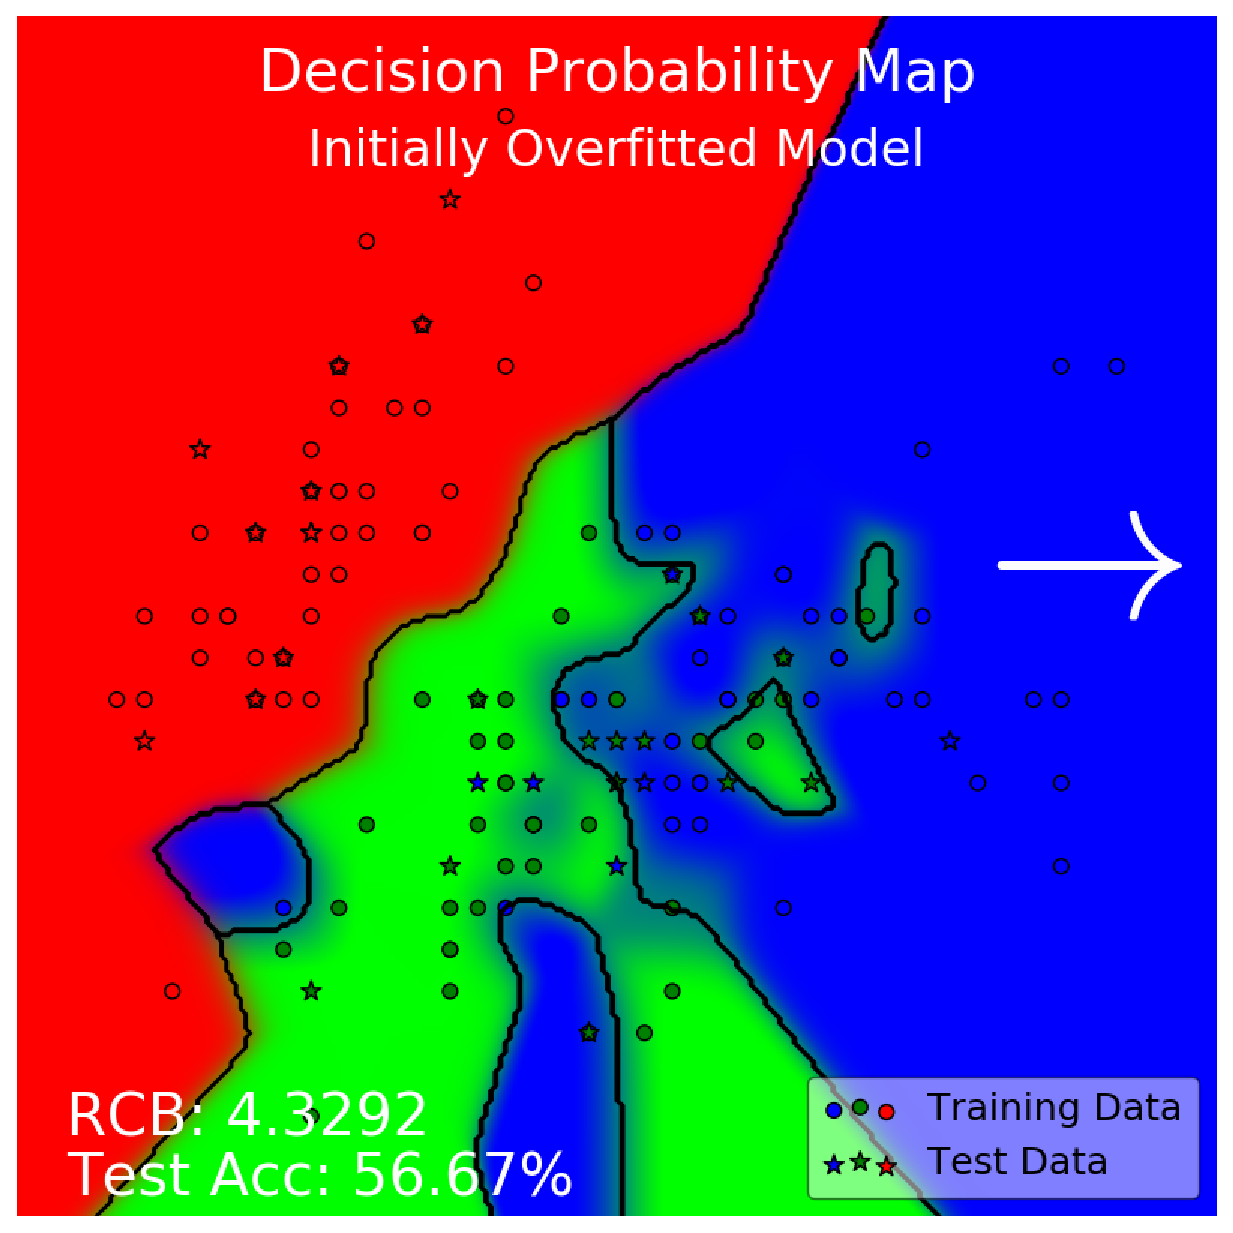
\includegraphics[width=0.32\linewidth]{figures/iris_overfitted_model.eps}
			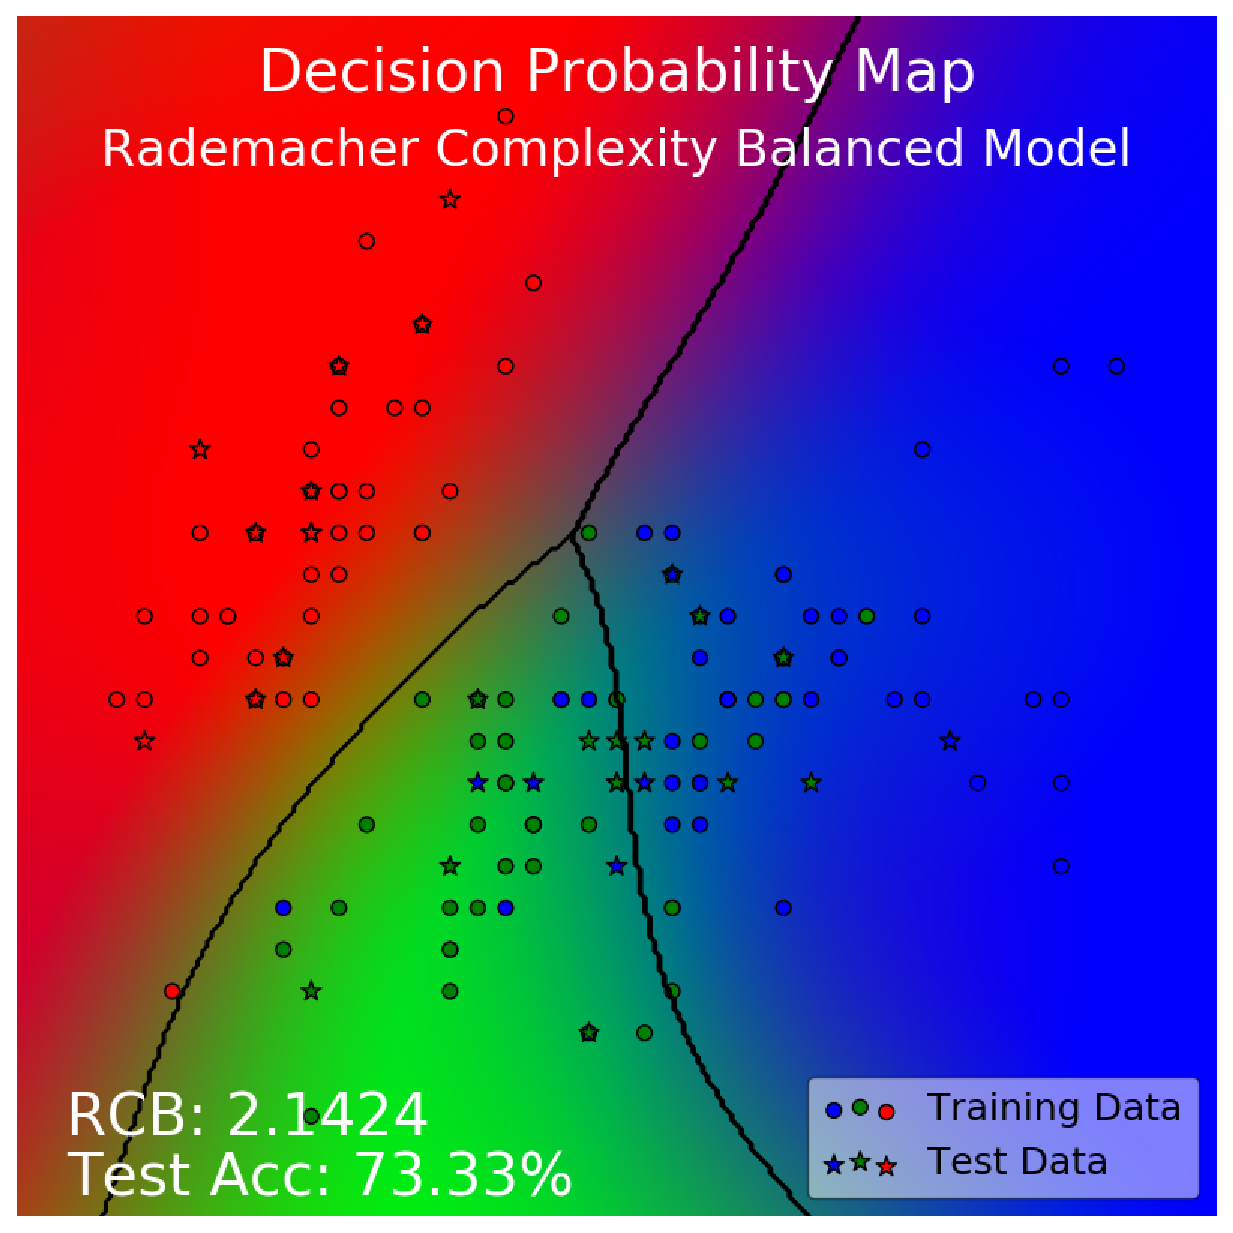
\includegraphics[width=0.32\linewidth]{figures/iris_balanced_model.eps}
			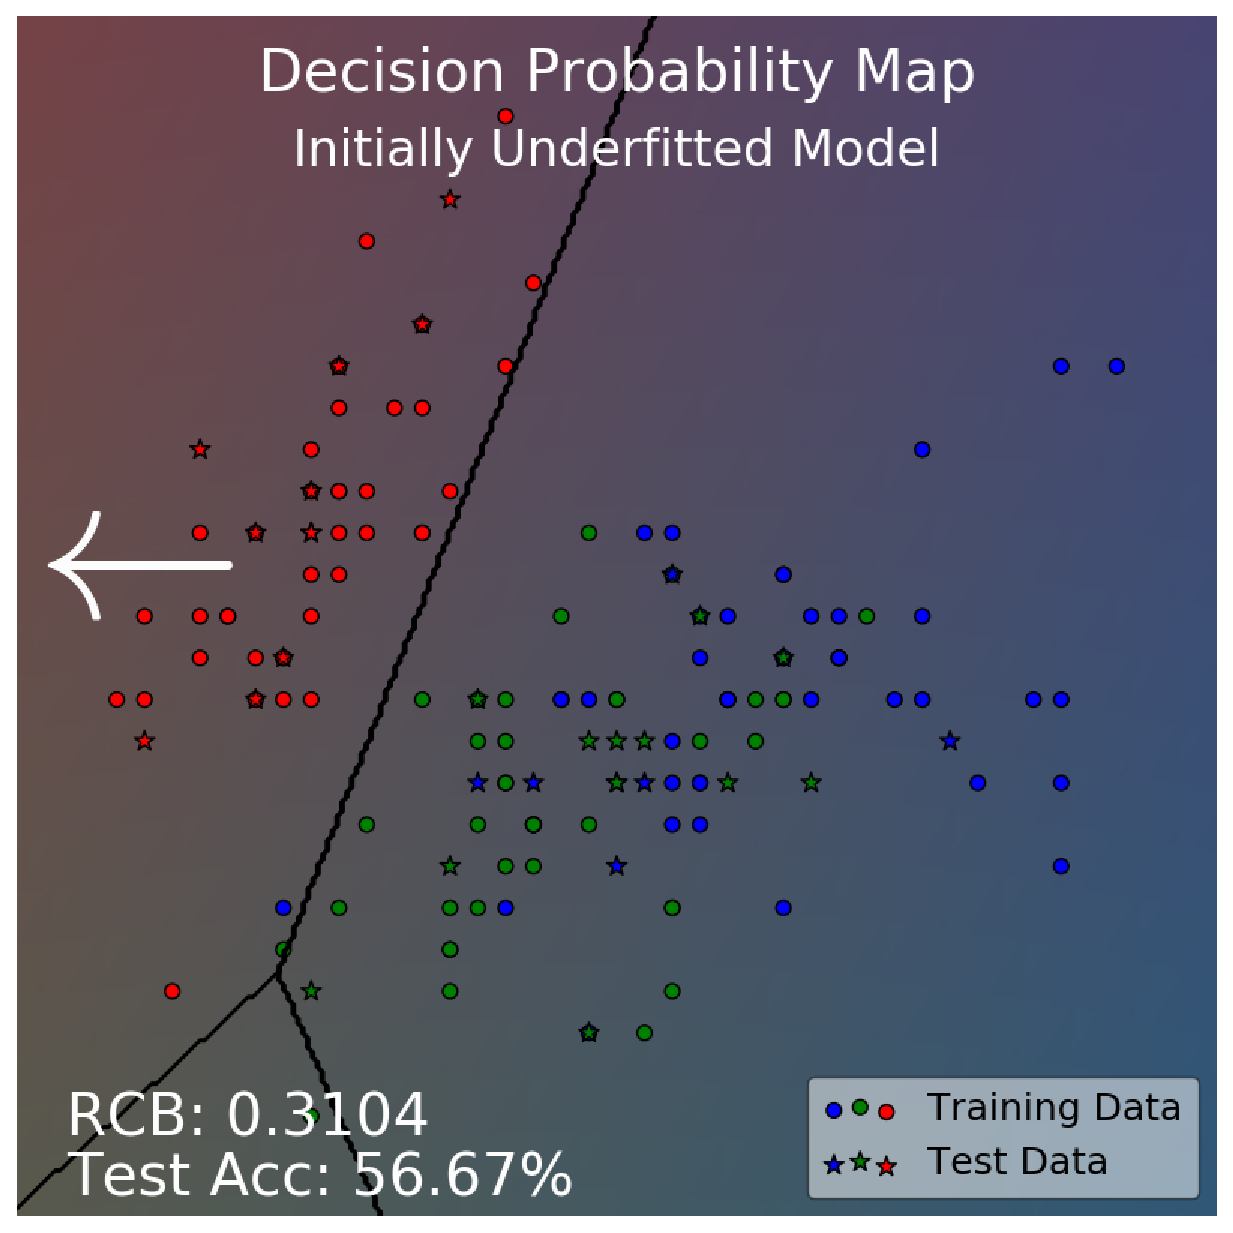
\includegraphics[width=0.32\linewidth]{figures/iris_underfitted_model.eps}
			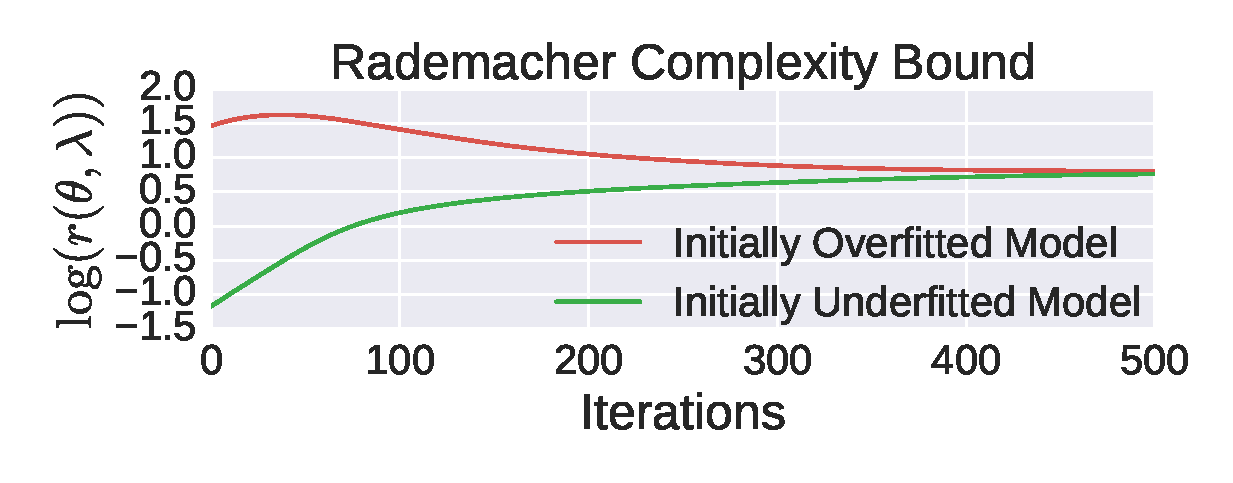
\includegraphics[width=0.48\linewidth]{figures/iris_rademacher_complexity_bound_lower_legend.eps}
	%		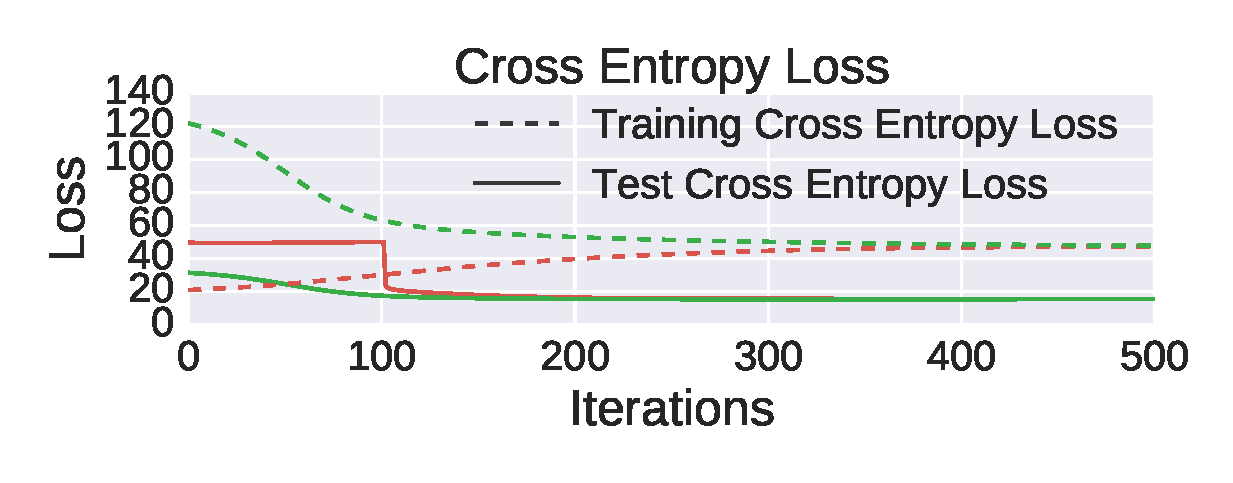
\includegraphics[width=0.48\linewidth]{figures/iris_cross_entropy_loss.eps}
			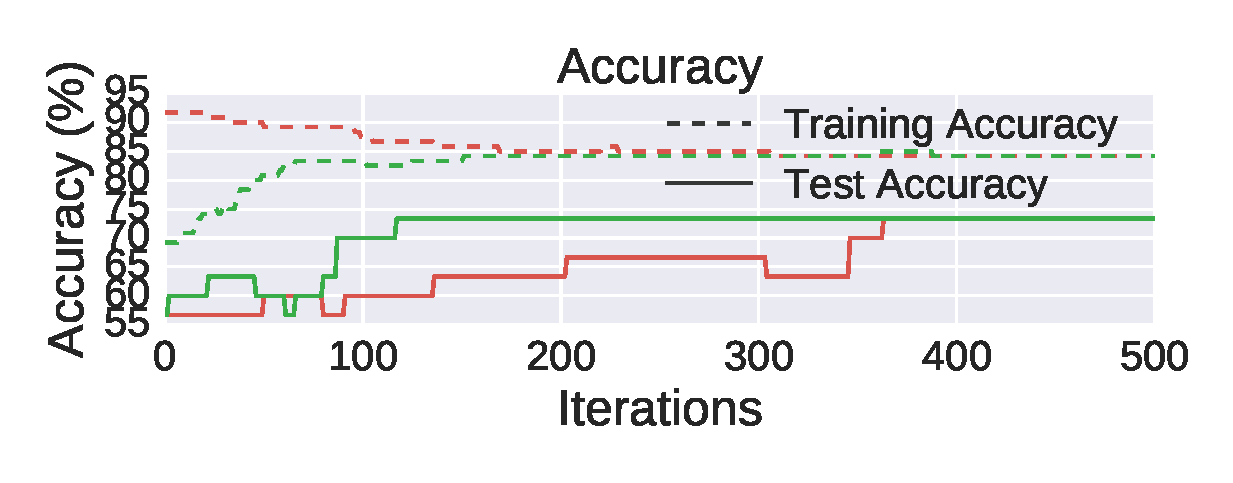
\includegraphics[width=0.48\linewidth]{figures/iris_accuracy.eps}
			\caption{Rademacher complexity balanced learning of hyperparameters for an isotropic Gaussian \gls{MCE}, using the first two attributes of the iris dataset.}
			\label{fig:iris}
		\end{figure*}
		
		The first two of four total attributes of the iris dataset \citep{fisher1936use} is known to have class labels that are not only not linearly separable, but also non-separable by any means, in that the same example $x \in \mathbb{R}^{2}$ may be assigned different output labels $y \in \mathbb{N}_{3} := \{1, 2, 3\}$ as they were only separable with the two remaining attributes. In these difficult scenarios, the notion of model complexity is extremely important, and the success of a learning algorithm greatly depends on how it balances training performance and model complexity to avoid both underfitting and overfitting. 
		
		\Cref{fig:iris} demonstrates \cref{alg:multiclass_conditional_embedding_training} with full gradient updates ($n_{b} = n$) to learn hyperparameters of the \gls{MCE} on the two attribute iris dataset. The kernel used is isotropic Gaussian with diagonal length scales $\Sigma = \ell^{2} I_{2}$ and sensitivity $\alpha = \sigma_{f}$, so the hyperparameters are $\theta = (\alpha, \ell)$ and $\lambda$. We evaluate the performance of the learning algorithm on a withheld test set using 20\% of the available 150 data samples. Attributes are scaled into the unit range $[0, 1]$ and decision probability maps are plotted for the region $[-0.5, 1.05]^{2}$, where the red, green, and blue colour channels represent the clip-normalized decision probability \eqref{eq:empirical_decision_probability_clip_normalised} for classes $c = 1, 2, 3$. We begin from two initial scenarios, one originally overfitting ($\alpha_{o} = 0.01$, $\ell_{o} = 0.035$, $\lambda_{o} = 10^{-6}$) and another underfitting ($\alpha_{u} = 1$, $\ell_{u} = 1$, $\lambda_{u} = 1$) the training data. Initially, both models performs sub-optimally with a test accuracy of 56.67\%. We see that the \gls{RCB} $r(\theta, \lambda)$ appropriately measures the amount of overfitting with $r((\alpha_{o}, \ell_{o}), \lambda_{o}) = 4.33$ and $r((\alpha_{u}, \ell_{u}), \lambda_{u}) = 0.31$. We then learn hyperparameters with \cref{alg:multiclass_conditional_embedding_training} for 500 iterations from both initializations at rate $\eta = 0.01$, where both models converges to a balanced model with appropriate \glspl{RCB} $r((\alpha_{o}, \ell_{o}), \lambda_{o}) = r((0.01, 0.24), 8.62 \times 10^{-7}) = 2.23 \approx 2.14 = r((\alpha_{u}, \ell_{u}), \lambda_{u}) = r((5.1, 0.24), 0.20)$ and an improved test accuracy of 73.33\%. In particular, the initially overfitted model learns a simpler model at the expense of lower training performance, emphasizing the benefits of complexity based regularization, without which the learning would only maximize training performance at the cost of further overfitting. Meanwhile, the initially underfitted model learns to increase complexity to improve the unflattering performance on the training set. In both scenarios, our learning algorithm improved performance on the test set.
	
	\paragraph{UCI Datasets}
	
		%	\begin{table*}[t]
		%		\caption{Classification accuracy (\%) on UCI datasets}
		%		\label{tab:uci_experiments}
		%		\centering
		%		\begin{tabular}{lcccccccc}	
		%			Dataset \hspace{\fill} $(n, d, m)$ & G\gls{MCE} & G\gls{MCE}-SGD & KEN-1 & KEN-2 & ERM & CV & MED & Others \\
		%			\midrule
		%			\texttt{banknote} \hspace{\fill} (1372, 4, 2) & $\mathbf{99.9 \pm 0.2}$ & $98.8 \pm 0.9$ & $99.5 \pm 1.0$ & $99.4 \pm 0.9$ & $\mathbf{99.9 \pm 0.2}$ & $\mathbf{99.9 \pm 0.2}$ & $92.0 \pm 4.3$ & 99.78\textsuperscript{a} \\
		%			\texttt{ecoli} \hspace{\fill} (336, 7, 8) & $\mathbf{87.5 \pm 4.4}$ & $84.5 \pm 5.0$ & $\mathbf{87.5 \pm 3.2}$ & $86.3 \pm 6.0$ & $72.1 \pm 20.5$ & $73.8 \pm 23.8$ & $42.1 \pm 47.7$ & 81.1\textsuperscript{b} \\
		%			\texttt{robot} \hspace{\fill} (5456, 24, 4) & $\mathbf{96.7 \pm 0.9}$ & $95.5 \pm 0.9$ & $82.3 \pm 7.1$ & $94.5 \pm 0.8$ & $91.0 \pm 3.7$ & $90.9 \pm 3.4$ & $81.1 \pm 6.2$ & 97.59\textsuperscript{c} \\
		%			\texttt{segment} \hspace{\fill} (2310, 19, 7) & $\mathbf{98.4 \pm 0.8}$ & $96.1 \pm 1.5$ & $94.6 \pm 1.6$ & $96.7 \pm 1.1$ & $98.1 \pm 1.1$ & $98.3 \pm 1.3$ & $27.3 \pm 26.4$ & 96.83\textsuperscript{d} \\
		%			\texttt{wine} \hspace{\fill} (178, 13, 3) & $\mathbf{97.2 \pm 3.7}$ & $93.3 \pm 6.0$ & $96.1 \pm 5.0$ & $97.2 \pm 5.1$ & $93.9 \pm 5.2$ & $93.3 \pm 7.4$ & $93.3 \pm 7.8$ & 100\textsuperscript{e} \\
		%			\texttt{yeast} \hspace{\fill} (1484, 8, 10) & $52.5 \pm 2.1$ & $\mathbf{60.3 \pm 4.4}$ & $55.8 \pm 5.0$ & $59.6 \pm 4.0$ & $45.9 \pm 6.4$ & $58.0 \pm 5.8$ & $31.2 \pm 14.1$ & 55.0\textsuperscript{b} \\
		%		\end{tabular}
		%	\end{table*}
		
		\begin{table*}[t]
			\caption{Test accuracy (\%) on UCI datasets}
			\label{tab:uci_experiments}
			\centering
			\begin{tabular}{lcccccccc}	
				Dataset & G\gls{MCE} & G\gls{MCE}-SGD & \gls{CEN}-1 & \gls{CEN}-2 & ERM & CV & MED & Others \\
				\midrule
				\texttt{banknote} & $\mathbf{99.9 \pm 0.2}$ & $98.8 \pm 0.9$ & $99.5 \pm 1.0$ & $99.4 \pm 0.9$ & $\mathbf{99.9 \pm 0.2}$ & $\mathbf{99.9 \pm 0.2}$ & $92.0 \pm 4.3$ & 99.78\textsuperscript{a} \\
				\texttt{ecoli} & $\mathbf{87.5 \pm 4.4}$ & $84.5 \pm 5.0$ & $\mathbf{87.5 \pm 3.2}$ & $86.3 \pm 6.0$ & $72.1 \pm 20.5$ & $73.8 \pm 23.8$ & $42.1 \pm 47.7$ & 81.1\textsuperscript{b} \\
				\texttt{robot} & $\mathbf{96.7 \pm 0.9}$ & $95.5 \pm 0.9$ & $82.3 \pm 7.1$ & $94.5 \pm 0.8$ & $91.0 \pm 3.7$ & $90.9 \pm 3.4$ & $81.1 \pm 6.2$ & 97.59\textsuperscript{c} \\
				\texttt{segment} & $\mathbf{98.4 \pm 0.8}$ & $96.1 \pm 1.5$ & $94.6 \pm 1.6$ & $96.7 \pm 1.1$ & $98.1 \pm 1.1$ & $98.3 \pm 1.3$ & $27.3 \pm 26.4$ & 96.83\textsuperscript{d} \\
				\texttt{wine} & $\mathbf{97.2 \pm 3.7}$ & $93.3 \pm 6.0$ & $96.1 \pm 5.0$ & $97.2 \pm 5.1$ & $93.9 \pm 5.2$ & $93.3 \pm 7.4$ & $93.3 \pm 7.8$ & 100\textsuperscript{e} \\
				\texttt{yeast} & $52.5 \pm 2.1$ & $\mathbf{60.3 \pm 4.4}$ & $55.8 \pm 5.0$ & $59.6 \pm 4.0$ & $45.9 \pm 6.4$ & $58.0 \pm 5.8$ & $31.2 \pm 14.1$ & 55.0\textsuperscript{b} \\
			\end{tabular}
		\end{table*}
		
		We demonstrate the average performance of learning anisotropic Gaussian kernels and kernels constructed from neural networks on standard UCI datasets \citep{bache2013uci}, summarized in \cref{tab:uci_experiments}. The former has a shallow but wide model architecture, while the latter has a deeper but narrower model architecture. The Gaussian kernel is learned with both full (G\gls{MCE}) and batch stochastic gradient updates (G\gls{MCE}-SGD) using a tenth ($n_{b} \approx \frac{n}{10}$) of the training set each training iteration, with sensitivity and length scales initialized to $1$. For \glspl{CEN}, we randomly select two simple fully connected architectures with 16-32-8 (\gls{CEN}-1) and 96-32 (\gls{CEN}-2) hidden units respectively, and learn the conditional embedding without dropout under ReLU activation. Biases and standard deviations of zero mean truncated normal distributed weights are initialized to $0.1$, and are to be learned with full gradient updates. For all experiments, $\lambda$ is initialized to $1$ and is learned jointly with the kernel. Optimization is performed with the Adam optimizer \citep{kingma2014adam} in TensorFlow \citep{abadi2016tensorflow} with rate $\eta = 0.1$ and $\epsilon = 10^{-15}$ under the learning objective $q(\theta, \lambda)$ \eqref{eq:learning_objective}. Learning is ran for 1000 epochs, regardless of convergence, for direct comparison. All attributes are scaled to the unit range. Each model is trained on 9 out of 10 folds and tested on the remaining fold, which are shuffled over all 10 combinations to obtain the test accuracy average and deviation. We compare our results to \glspl{MCE} whose hyperparameters are tuned by \gls{ERM}, cross validation (CV), and the median heuristic (MED), as well as to other approaches using neural networks \citep[a; c]{kaya2016banknote, freire2009short}, probabilistic binary trees \citep[b]{horton1996probabilistic}, decision trees \citep[d]{zhou2004size}, and regularised discriminant analysis \citep[e]{aeberhard1992comparison}. \Cref{tab:uci_experiments} shows that our learning algorithm outperforms other hyperparameter tuning algorithms, and performs similarly to competing methods. Our method achieves this without any special tuning or heuristics, but by simply placing a conditional embedding on training data and applying a complexity bound based learning algorithm. The stochastic gradient approach for Gaussian kernels performs similarly to the full gradient approach, supporting \cref{thm:expected_risk_bound_hyperparameter_learning_copy} for $n = n_{b}$. For \glspl{CEN}, we did not attempt to choose an optimal architecture for each dataset. The learning algorithm is to train the same simple untrained network for different datasets under only 1000 epochs, and still generates comparable performance. 
	
	\paragraph{MNIST by learning pixel length scales}
	
		We apply \cref{alg:multiclass_conditional_embedding_training} to learn anisotropic length scales of Gaussian kernels on pixels of the MNIST digits dataset \citep{lecun1998gradient}. In the top left plot of \cref{fig:mnist_experiments}, we train on datasets of varying sizes, from 50 to 5000 images, and benchmark performance on the standard test set of 10000 images. All hyperparameters are initialized to 1 before learning. We train both \glspl{SVC} and \glspl{GPC} under the \gls{OVA} scheme, and use a Laplace approximation for the \gls{GPC} posterior. In all cases, \glspl{MCE} outperform \glspl{SVC}, as standard \gls{SVC} training cannot learn hyperparameters unless expensive cross validation is performed. \glspl{MCE} also outperform \glspl{GPC} as more data becomes available. Under the \gls{OVA} scheme, a set of kernel hyperparameters are learned to distinguish each class against the rest, while for our algorithm learns a consistent set of hyperparameters for all classes. Consequently, for 5000 data points, the computational time required for hyperparameter learning of standard \glspl{GPC} is on the order of days, while \cref{alg:multiclass_conditional_embedding_training} is on the order of hours even without batch updates. We also compare hyperparameter learning with and without the \gls{RCB}. For small $n$ below 750 samples, the latter outperforms the former (e.g. 86.69\% and 86.96\% for $n = 500$), while for large $n$ the former outperforms the latter (e.g. 96.05\% and 95.3\% for $n= 5000$). This verifies that complexity based regularization becomes especially important as data size grows, when overfitting starts to hurt generalization performance. Our bound is also tighter with larger $n$, so that generalization performance improves with more data. The images at the bottom of \cref{fig:mnist_experiments} show the pixel length scales learned through batch stochastic gradient updates ($n_{b} = 1200$) on all available training images of different groups of digits, demonstrating the most discriminative regions for classification. %In particular, the most discriminative regions are usually around the edges of the digits, subject to slight intraclass translations. 
	
		% % % Removed sentences
		% We first demonstrate the test performance of \glspl{MCE} as the training set increases in size, verifying \cref{thm:probability_convergence_copy} in that decision probabilities converge to the true and thus test distribution as $n$ increases.
		% The MNIST dataset has $d = 28^{2} = 784$ pixel dimensions, yet with only $n = 50, 150, 250$ training samples, the \gls{MCE} achieves a test accuracy of 45.7\%, 70.09\%, and 79.37\% respectively, compared to 18.13\%, 37.43\%, and 53.81\% from SVCs.

	\paragraph{MNIST by learning convolutional features}
	
		\begin{figure*}[t]
			\centering 
			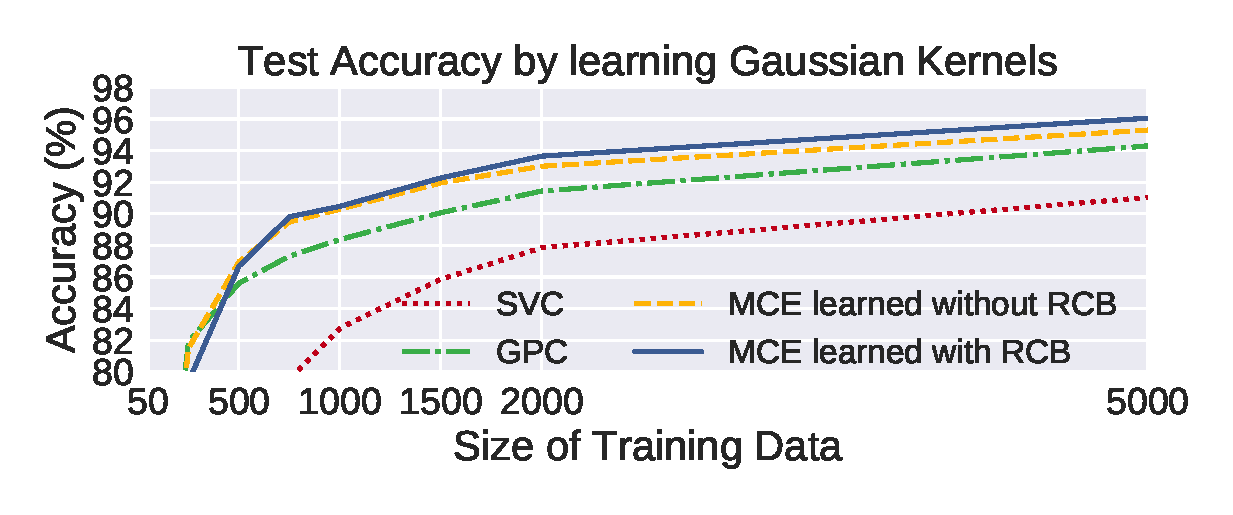
\includegraphics[width=0.49\linewidth]{figures/gaussian_mnist_test_performance_short.eps}
			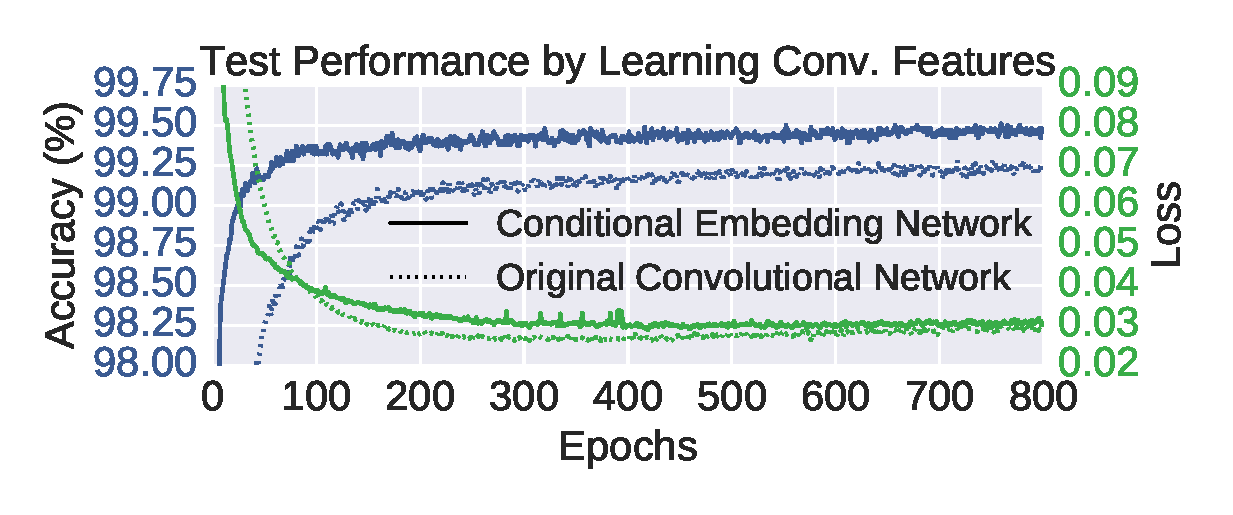
\includegraphics[width=0.49\linewidth]{figures/deep_mnist_test_performance_short.eps}
			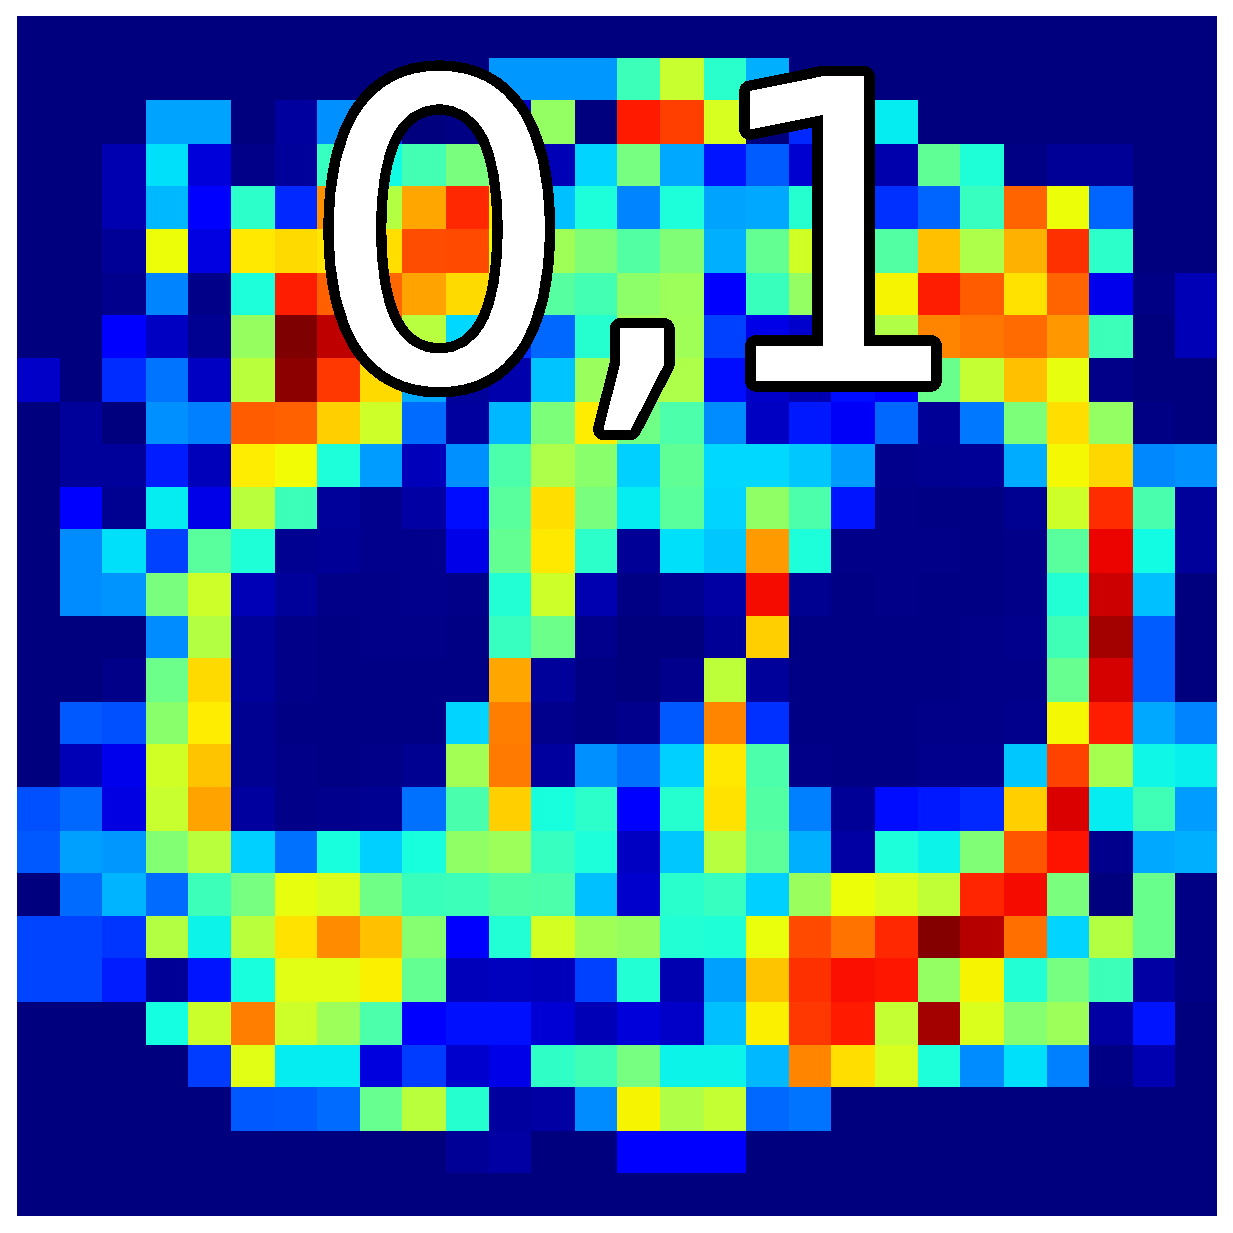
\includegraphics[width=0.1\linewidth]{figures/pixel_relevance_01_batch_1200.eps}
			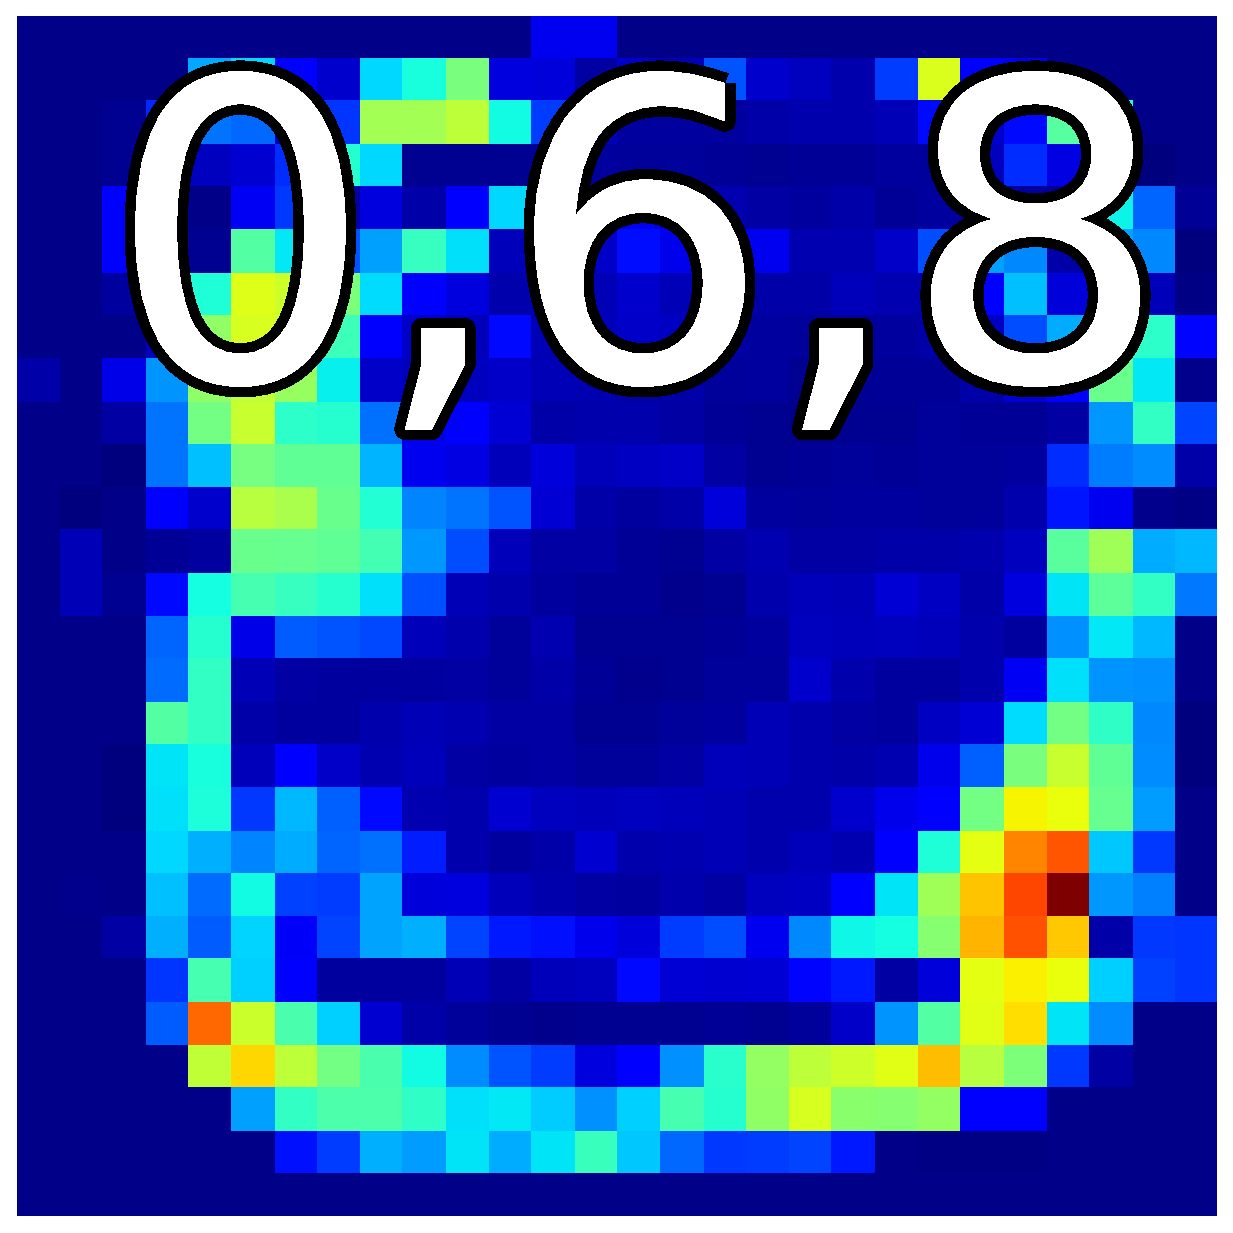
\includegraphics[width=0.1\linewidth]{figures/pixel_relevance_068_batch_1200.eps}
			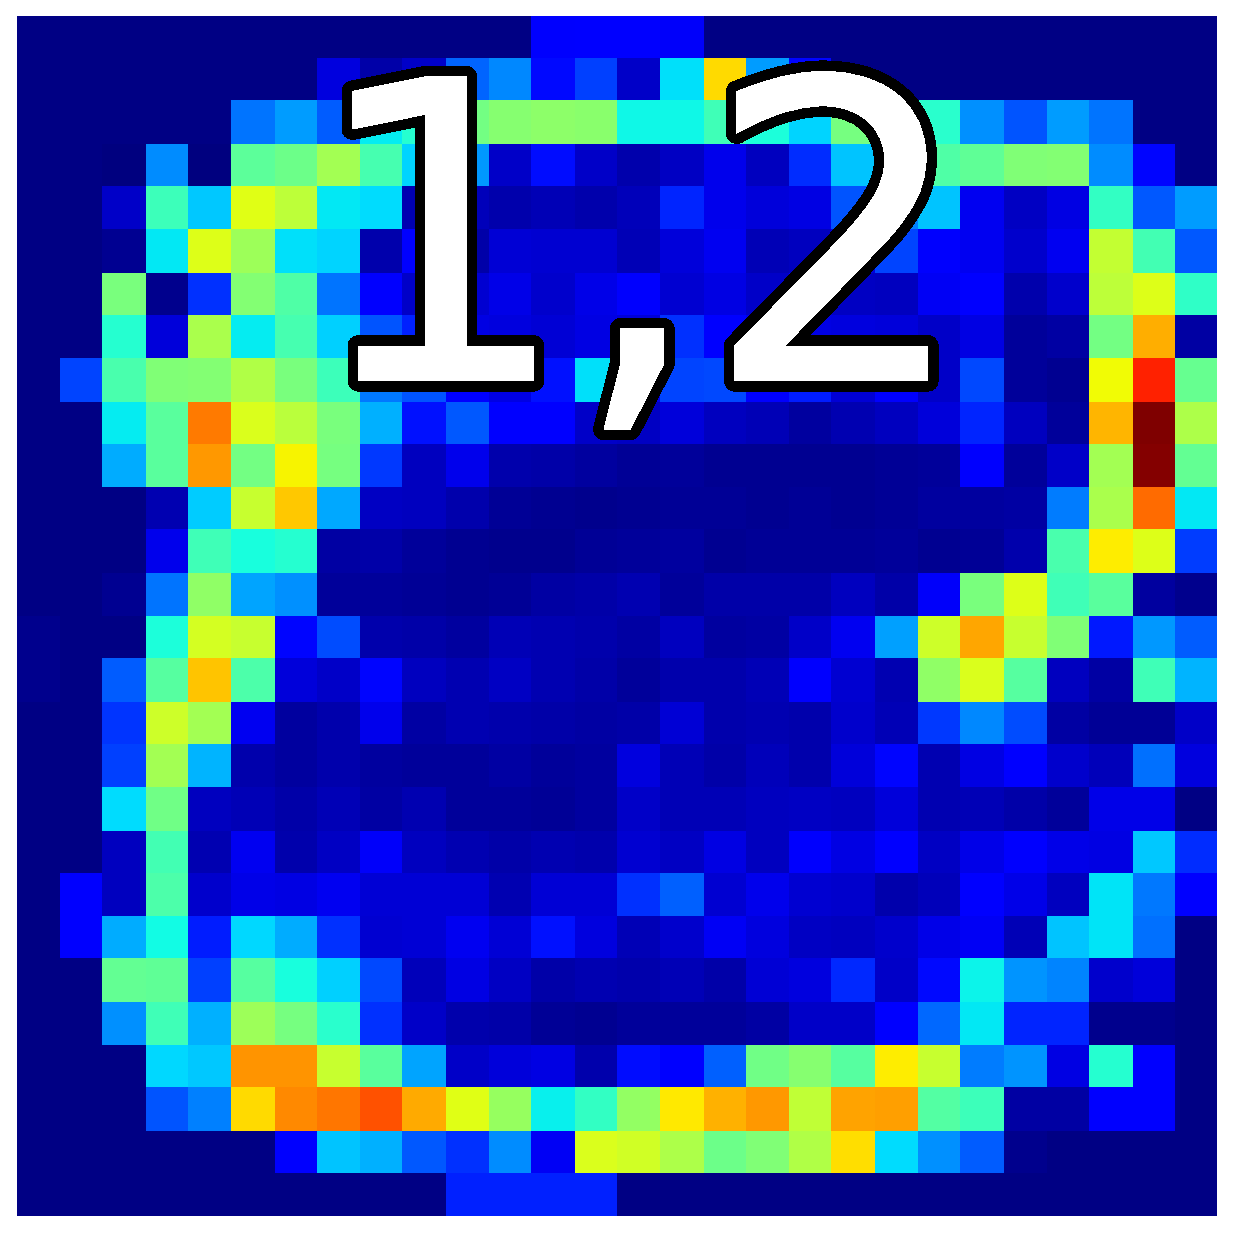
\includegraphics[width=0.1\linewidth]{figures/pixel_relevance_12_batch_1200.eps}
			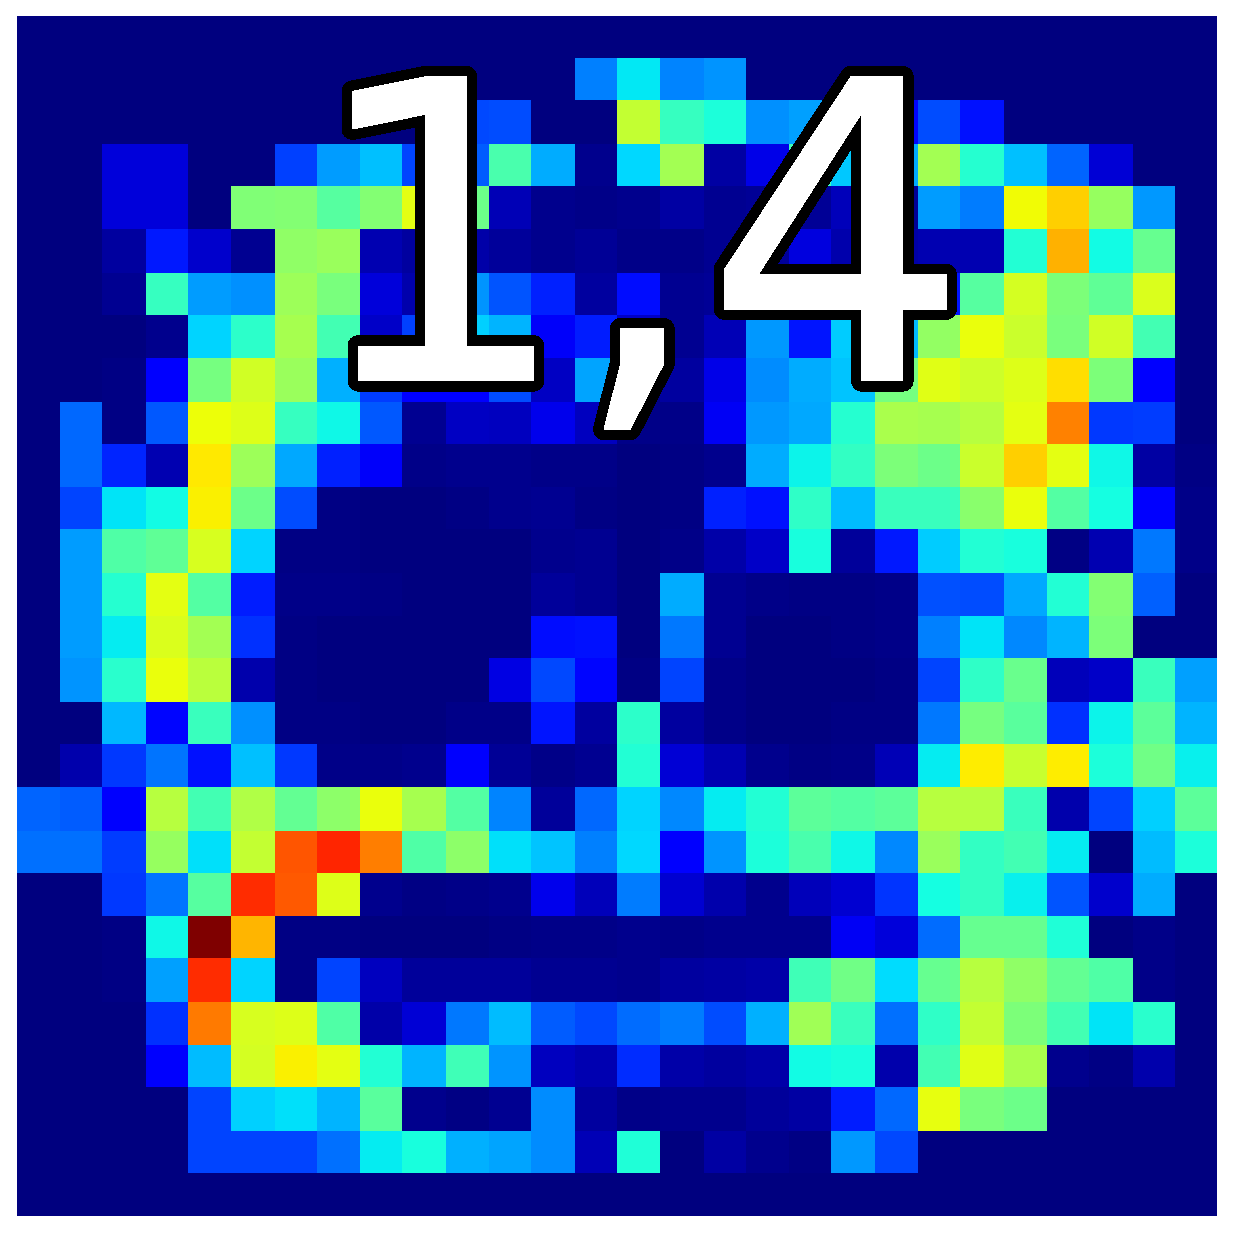
\includegraphics[width=0.1\linewidth]{figures/pixel_relevance_14_batch_1200.eps}
			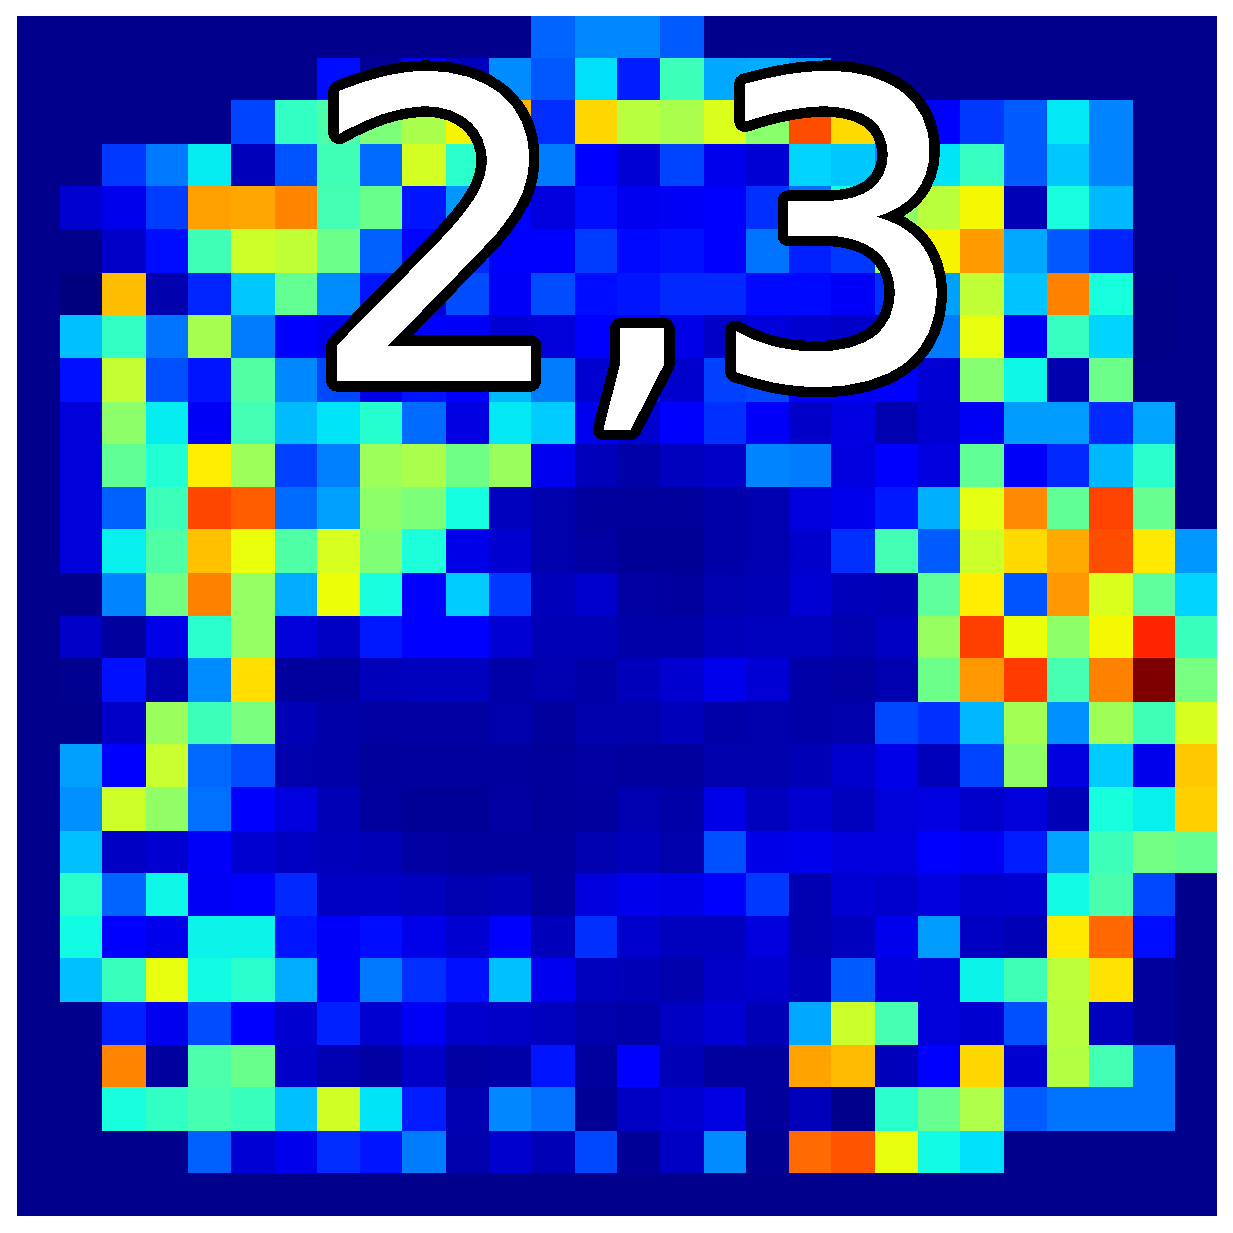
\includegraphics[width=0.1\linewidth]{figures/pixel_relevance_23_batch_1200.eps}
			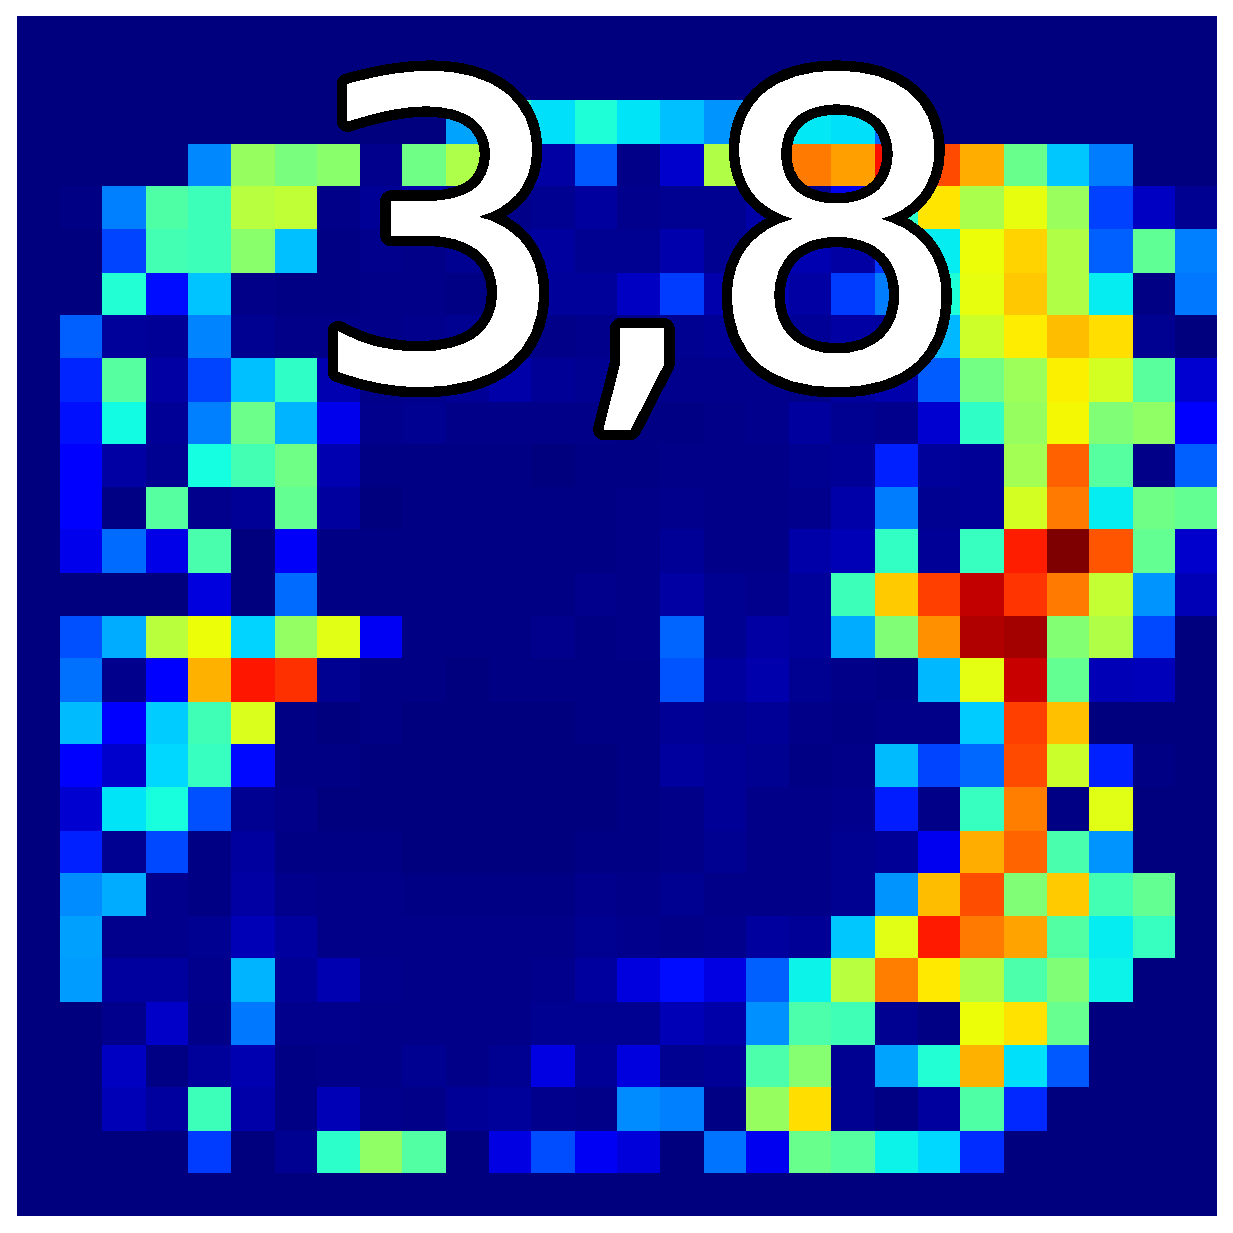
\includegraphics[width=0.1\linewidth]{figures/pixel_relevance_38_batch_1200.eps}
			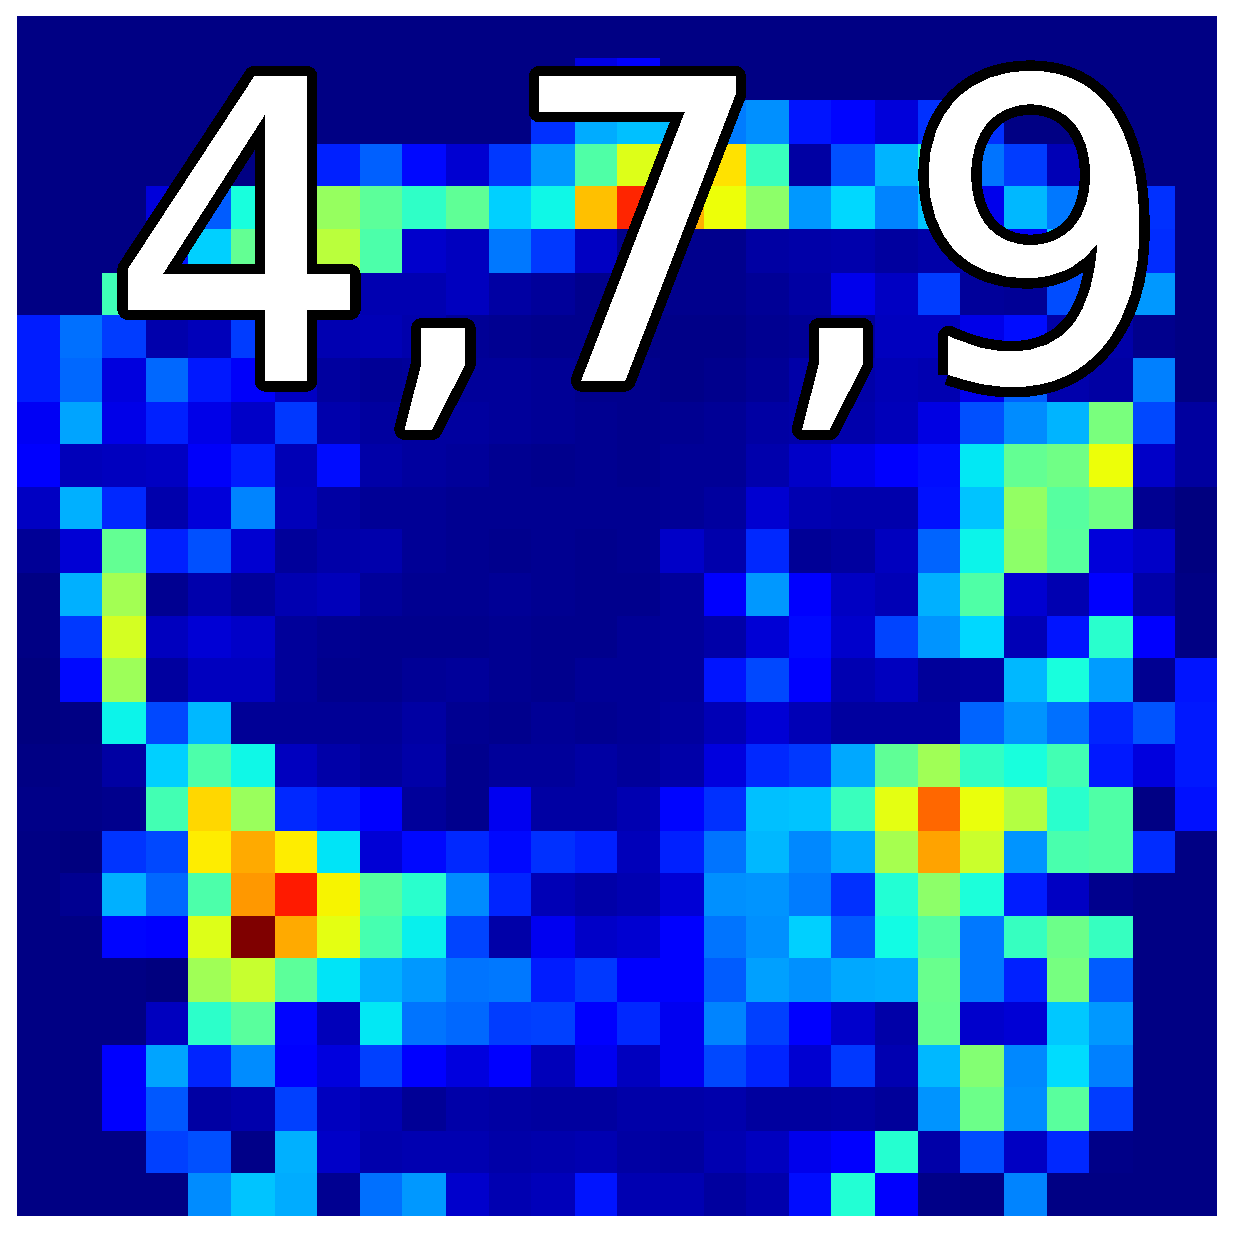
\includegraphics[width=0.1\linewidth]{figures/pixel_relevance_479_batch_1200.eps}
			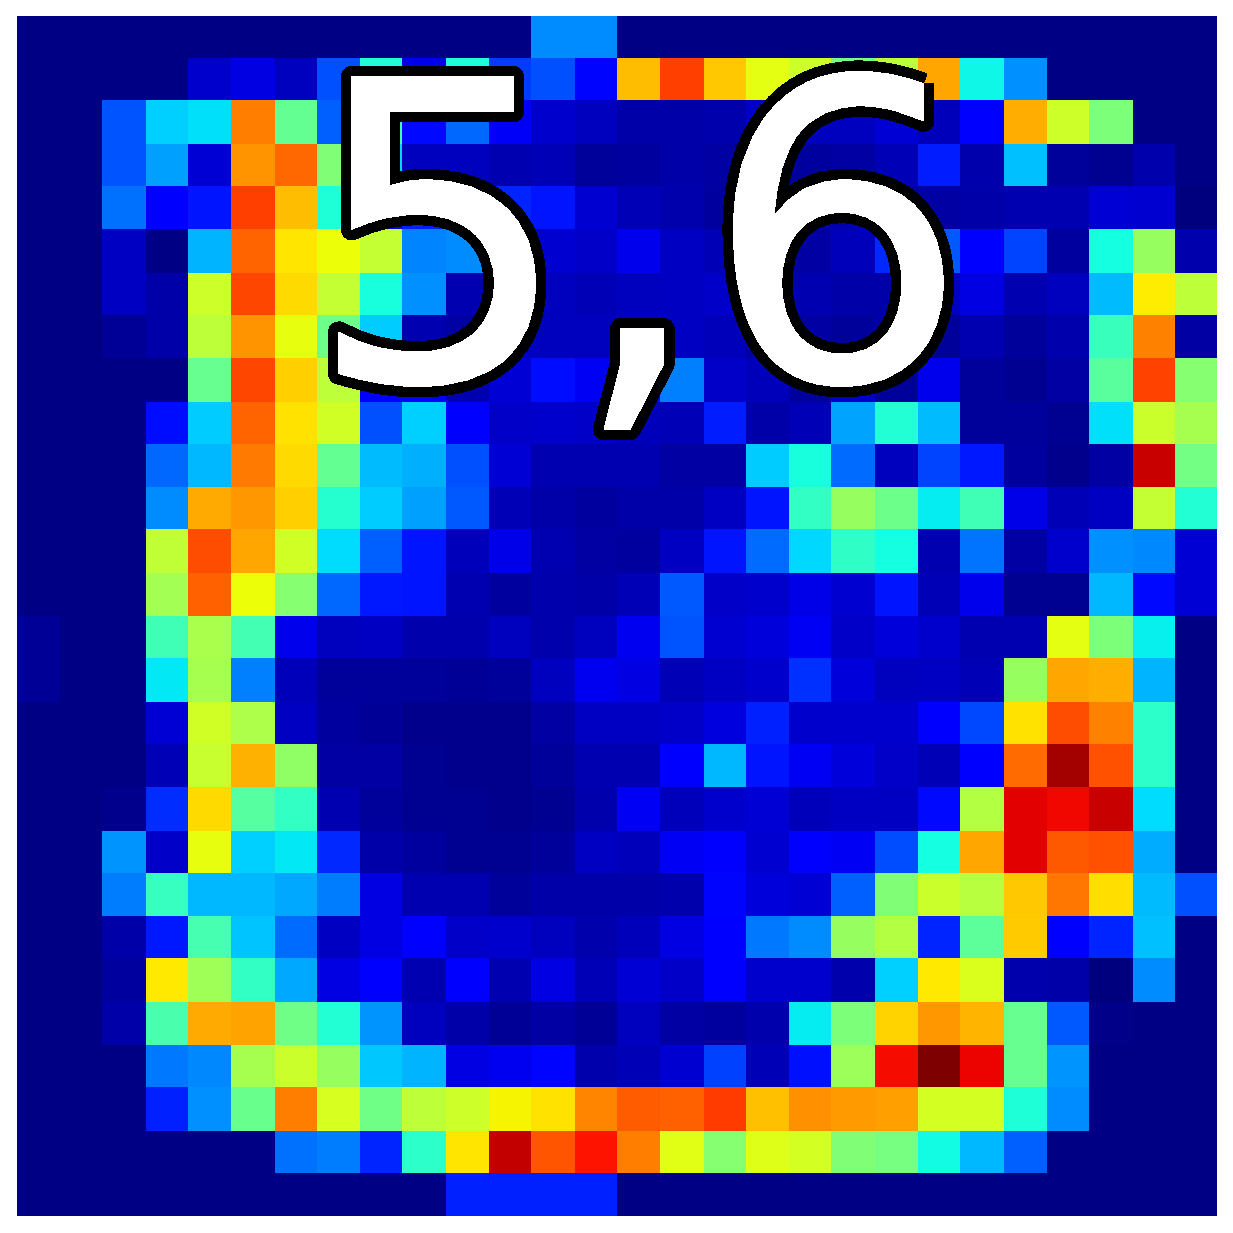
\includegraphics[width=0.1\linewidth]{figures/pixel_relevance_56_batch_1200.eps}
			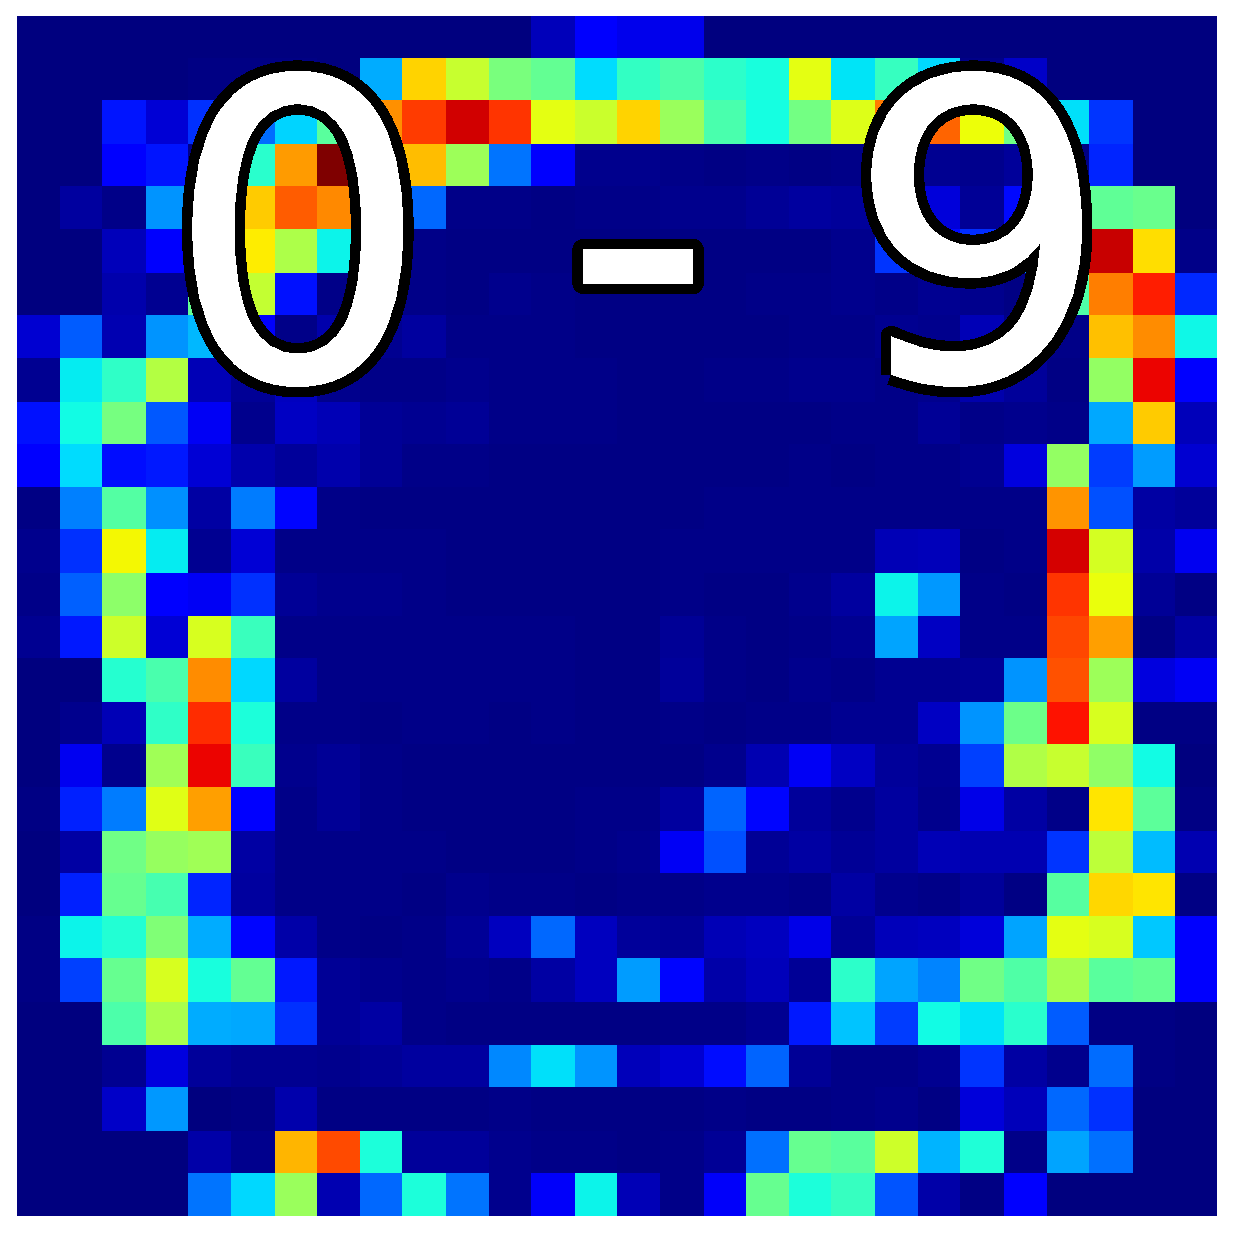
\includegraphics[width=0.1\linewidth]{figures/pixel_relevance_0123456789_batch_1200.eps}
			\caption{Top: Test accuracy by learning Gaussian kernels (left) and deep convolutional features (right). Bottom: Learned pixel length scales under anistropic Gaussian (ARD) kernels.}
			\label{fig:mnist_experiments}
		\end{figure*}
		
		We now apply our learning algorithm to train \gls{CNN} on the MNIST dataset. We employ an example architecture from the TensorFlow tutorial on deep MNIST classification \citep{abadi2016tensorflow}. This ReLU activated architecture uses two convolutional layers, each with max pooling, followed by a fully connected layer with a drop out probability of 0.5. The original network then employs a final softmax regressor on the last hidden layer for classification. The \gls{CEN} instead employs a linear kernel on the last hidden layer to construct the conditional embedding. We then train both networks from the same initialization with batch updates using $n_{b} = 6000$ images at a time for 800 epochs, with learning rate $\eta = 0.01$. All biases and standard deviations of zero mean truncated normal distributed weights are initialized to 0.1. The network weights and biases of the \gls{CEN} are learned jointly with the regularization parameter, initialized to $\lambda = 10$, under our learning objective \eqref{eq:learning_objective}, while the original \gls{CNN} is trained under its usual cross entropy loss. The fully connected layer is trained with a drop out probability of 0.5 for both cases to allow direct comparison. The top right plot in \cref{fig:mnist_experiments} shows that \glspl{CEN} learns at a much faster rate, maintaining a higher test accuracy at all epochs. After 800 epochs, \gls{CEN} reaches a test accuracy of 99.48\%, compared to 99.26\% from the original \gls{CNN}. This demonstrates that our learning algorithm can perform end-to-end learning with \glspl{CNN} from scratch, by simply replacing the softmax layer with an \gls{MCE}. The resulting \gls{CEN} can outperform the original \gls{CNN} in both convergence rate and accuracy.
	
	\section{Conclusion}
	
		We propose a scalable hyperparameter learning framework for \glspl{MCE}. Because nonparametric models have infinite capacity and can potentially overfit, we derive learning-theoretic bounds to regularize the \gls{MCE} in a way that minimizes expected generalization risk. The resulting bound justifies the use of stochastic gradient updates for hyperparameter learning, which we verify experimentally. Our algorithm does not impose restrictions to the form of the positive definite kernel, and in particular can perform end-to-end learning on a neural network by replacing the softmax layer with a \gls{MCE}, which we demonstrate on UCI datasets and MNIST digits, where it outperforms the original convolutional neural network in the latter.
		
		This framework can incorporated and extended in many ways into techniques that requires appropriately learned conditional embeddings. In particular, nonparametric probabilistic inference can be carried out in the \gls{RKHS} to obtain joint and reverse conditional embeddings, where mode decoding, density recovery, and sampling techniques can lead to effective generative models now that hyperparameters are learned. This line of approach can potentially lead to Bayesian extensions to our framework. We also envision a semi-supervised and one class extension to the \gls{MCE} framework that can relax supervision in training. Moreover, instead of a Kronecker delta kernel, kernels in the label space with non-zero and potentially learnable similarities between distinct labels may capture label correlations better than our original framework. Finally, our framework and algorithm is simple, and developments in establishing deeper connections and relationships with other kernel based models can be fruitful. 
	
	\newpage
	\bibliography{kernel_embedding}
	\bibliographystyle{apalike}

\end{document}

